% !TeX program = pdflatex
%=======================================================================
%  Informe generado desde source/informe.md por tools/md2report.py
%  Compilar:  pdflatex informe.tex  (tres veces, por el indice)
%=======================================================================
\documentclass[11pt,a4paper]{article}

\usepackage[T1]{fontenc}
\usepackage[utf8]{inputenc}
\usepackage[spanish,es-noshorthands,es-tabla]{babel}
\usepackage{lmodern}
\usepackage[a4paper,top=2.5cm,bottom=2.4cm,left=2.8cm,right=2.5cm]{geometry}

\usepackage{xcolor}
\usepackage{graphicx}
\usepackage{booktabs}
\usepackage{longtable}
\usepackage{pdflscape}
\usepackage{array}
\usepackage{ragged2e}
\usepackage{enumitem}
\usepackage{amssymb}
\usepackage{titlesec}
\usepackage{fancyhdr}
\usepackage{parskip}
\usepackage{microtype}
\usepackage{caption}
\usepackage{etoolbox}
\usepackage[most]{tcolorbox}
\usepackage[hidelinks,breaklinks=true]{hyperref}
\usepackage{url}

\definecolor{navy}{HTML}{14496B}
\definecolor{sblue}{HTML}{2A78D6}
\definecolor{lblue}{HTML}{DCE8F4}
\definecolor{lgray}{HTML}{E6E8EA}
\definecolor{lamber}{HTML}{FBF1DE}
\definecolor{amber}{HTML}{A6690C}
\definecolor{red}{HTML}{B23B32}
\definecolor{green}{HTML}{2C6A49}
\definecolor{ink}{HTML}{18222E}
\definecolor{gray2}{HTML}{6D7885}
\definecolor{rule2}{HTML}{CFD5DC}
\definecolor{navybg}{HTML}{EFF4F9}
\definecolor{amberbg}{HTML}{FDF7EC}
\definecolor{redbg}{HTML}{FDF4F3}
\definecolor{greenbg}{HTML}{F1F7F3}

\hypersetup{colorlinks=true, linkcolor=navy, urlcolor=navy,
            citecolor=navy, pdftitle={Oportunidades de robótica de inspección industrial para generación y utilities}}
\renewcommand{\UrlFont}{\small\ttfamily}
\Urlmuskip=0mu plus 1mu
\def\UrlBreaks{\do\/\do\-\do\_\do\.\do\=\do\&\do\?\do\#\do\:\do\0\do\1\do\2\do\3\do\4\do\5\do\6\do\7\do\8\do\9}
\sloppy

\newlength{\colw}
\newcolumntype{L}{>{\RaggedRight\arraybackslash}p{\colw}}
\renewcommand{\arraystretch}{1.3}
\setlist{topsep=3pt, itemsep=1.5pt, parsep=0pt, leftmargin=1.4em}
\captionsetup{skip=4pt}

% --- titulos ----------------------------------------------------------
\titleformat{\section}
  {\sffamily\LARGE\bfseries\color{navy}}{}{0pt}{}
  [\vspace{2pt}{\color{navy}\titlerule[1.4pt]}]
\titleformat{\subsection}{\sffamily\large\bfseries}{}{0pt}{}
  [\vspace{1pt}{\color{rule2}\titlerule[0.5pt]}]
\titleformat{\subsubsection}{\sffamily\normalsize\bfseries\color{navy}}{}{0pt}{}
\titleformat{\paragraph}[runin]{\sffamily\small\bfseries\color{gray2}}{}{0pt}{}[\quad]
\titlespacing*{\section}{0pt}{0pt}{14pt}
\titlespacing*{\subsection}{0pt}{18pt}{7pt}
\titlespacing*{\subsubsection}{0pt}{13pt}{4pt}

\pagestyle{fancy}
\fancyhf{}
\renewcommand{\headrulewidth}{0.4pt}
\fancyhead[L]{\sffamily\footnotesize\color{gray2}Oportunidades de robótica de
  inspección industrial para generación y utilities}
\fancyfoot[C]{\sffamily\footnotesize\thepage}

% --- distintivos ------------------------------------------------------
\newcommand{\badge}[3]{%
  \tcbox[on line, boxsep=1pt, left=2pt, right=2pt, top=0.5pt, bottom=0.5pt,
         colback=#1, colframe=#1, arc=1pt, boxrule=0pt]%
    {\color{#2}\sffamily\scriptsize\bfseries #3}}

% --- llamados ---------------------------------------------------------
\newtcolorbox{notaclavebase}{enhanced, breakable, sharp corners, boxrule=0pt,
  leftrule=2.5pt, colframe=amber, colback=amberbg,
  left=8pt, right=8pt, top=7pt, bottom=7pt, before skip=10pt, after skip=10pt}
\newenvironment{notaclave}[1]
  {\begin{notaclavebase}{\sffamily\scriptsize\bfseries\color{amber}#1}\par\vspace{2pt}}
  {\end{notaclavebase}}
\newtcolorbox{notadatobase}{enhanced, breakable, sharp corners, boxrule=0pt,
  leftrule=2.5pt, colframe=navy, colback=navybg,
  left=8pt, right=8pt, top=7pt, bottom=7pt, before skip=10pt, after skip=10pt}
\newenvironment{notadato}[1]
  {\begin{notadatobase}{\sffamily\scriptsize\bfseries\color{navy}#1}\par\vspace{2pt}}
  {\end{notadatobase}}
\newtcolorbox{notariesgobase}{enhanced, breakable, sharp corners, boxrule=0pt,
  leftrule=2.5pt, colframe=red, colback=redbg,
  left=8pt, right=8pt, top=7pt, bottom=7pt, before skip=10pt, after skip=10pt}
\newenvironment{notariesgo}[1]
  {\begin{notariesgobase}{\sffamily\scriptsize\bfseries\color{red}#1}\par\vspace{2pt}}
  {\end{notariesgobase}}
\newtcolorbox{notainferenciabase}{enhanced, breakable, sharp corners, boxrule=0pt,
  leftrule=2.5pt, colframe=green, colback=greenbg,
  left=8pt, right=8pt, top=7pt, bottom=7pt, before skip=10pt, after skip=10pt}
\newenvironment{notainferencia}[1]
  {\begin{notainferenciabase}{\sffamily\scriptsize\bfseries\color{green}#1}\par\vspace{2pt}}
  {\end{notainferenciabase}}

% --- tarjetas ---------------------------------------------------------
\newtcolorbox{tarjetabase}{enhanced, breakable, colframe=rule2, colback=white,
  boxrule=0.6pt, arc=2pt, left=8pt, right=8pt, top=6pt, bottom=6pt,
  before skip=8pt, after skip=8pt}
\newenvironment{tarjeta}[2]
  {\begin{tarjetabase}%
   {\sffamily\bfseries\color{navy}#1}%
   \ifstrempty{#2}{}{\\[1pt]{\sffamily\scriptsize\color{gray2}#2}}%
   \par\vspace{3pt}}
  {\end{tarjetabase}}

% --- desplegables (siempre visibles en papel) -------------------------
\newtcolorbox{detallebase}[1]{enhanced, breakable, colframe=rule2,
  colback=white, boxrule=0.6pt, arc=2pt, left=8pt, right=8pt, top=6pt,
  bottom=6pt, before skip=10pt, after skip=10pt,
  title={\sffamily\small\bfseries #1}, colbacktitle=navybg, coltitle=navy,
  titlerule=0pt}
\newenvironment{detalle}[1]{\begin{detallebase}{#1}}{\end{detallebase}}

\begin{document}
\pagenumbering{roman}

\begin{titlepage}
\thispagestyle{empty}
\setlength{\parindent}{0pt}\raggedright
\vspace*{3cm}
{\sffamily\footnotesize\bfseries\color{navy}\MakeUppercase{Edición 2026 \textperiodcentered{} Documento de trabajo para decisión de inversión}\par}
\vspace{8pt}
{\color{navy}\rule{\linewidth}{2.5pt}}
\vspace{22pt}

{\sffamily\huge\bfseries Oportunidades de robótica de inspección industrial para generación y utilities\par}
\vspace{14pt}
{\sffamily\large\color{gray2} Marco de evaluación, mapa de candidatos y plan de verificación\par}
\vspace{30pt}
{\color{rule2}\rule{0.35\linewidth}{0.6pt}\par}
\vspace{12pt}
{\normalsize Fecha de corte de la evidencia recopilada: 31 de agosto de 2026\par}
\vfill
{\sffamily\footnotesize\color{gray2}Documento de trabajo para decisión de
inversión. Las hipótesis y las fuentes recopiladas no constituyen conclusiones
de investigación mientras no estén verificadas.\par}
\end{titlepage}
\setcounter{page}{2}

\tableofcontents
\clearpage
\pagenumbering{arabic}

\clearpage

\section*{Resumen ejecutivo}
\addcontentsline{toc}{section}{Resumen ejecutivo}

Este documento define \textbf{qué robot de inspección industrial conviene desarrollar como próximo producto}, con qué evidencia se decide y qué queda por verificar antes de comprometer inversión. No es un catálogo de ideas técnicas: es el marco de decisión, el mapa de las siete oportunidades candidatas y el plan de verificación que las confirma o las descarta.

\begin{notadato}{Cómo leer este informe}
Los términos de negocio y del sector están definidos en el \textbf{Anexo C}, cada uno con la fuente donde puede verificarse la definición. En el texto, la primera aparición de cada término enlaza a su entrada. Cuando un término no tiene definición normativa, el anexo lo declara como definición operativa de este informe en lugar de atribuirle una fuente inexistente.

Las afirmaciones llevan su clase: \badge{navy}{white}{A} a \badge{lgray}{ink}{D} indican el nivel de la fuente, \badge{lamber}{amber}{Declaración} señala una afirmación comercial del fabricante no verificada de forma independiente, y \badge{lblue}{ink}{M4} indica madurez comercial en la escala de la sección 3.4.

\end{notadato}
\begin{notaclave}{La pregunta que ordena todo el estudio}
No se busca responder \emph{qué robots interesantes podrían construirse}, sino:

\textbf{¿En qué tareas de inspección o mantenimiento existe un dolor económico suficientemente grande, un acceso suficientemente difícil y un mercado suficientemente abierto como para justificar el desarrollo de un robot industrial especializado y construir un negocio rentable alrededor de él?}

\end{notaclave}

\subsection*{Estado de la evidencia al cierre de esta edición}
\addcontentsline{toc}{subsection}{Estado de la evidencia al cierre de esta edición}

\begin{center}\setlength{\tabcolsep}{4pt}
\begin{tabular}{>{\raggedright\arraybackslash}p{0.235\linewidth}>{\raggedright\arraybackslash}p{0.235\linewidth}>{\raggedright\arraybackslash}p{0.235\linewidth}>{\raggedright\arraybackslash}p{0.235\linewidth}}
{\color{navy}\Large\bfseries 8}\\[2pt]{\small candidatos con ficha de evaluación}\\[1pt]{\footnotesize\color{gray2} uno de ellos surgido del barrido ampliado} & {\color{navy}\Large\bfseries 3}\\[2pt]{\small con valor económico publicado}\\[1pt]{\footnotesize\color{gray2} por fuente de nivel A} & {\color{navy}\Large\bfseries 2}\\[2pt]{\small con incumbente comercial identificado}\\[1pt]{\footnotesize\color{gray2} TesTex en HRSG, Diakont en piping} & {\color{navy}\Large\bfseries 6}\\[2pt]{\small familias de activos descartadas con evidencia}\\[1pt]{\footnotesize\color{gray2} y registradas con su fuente} \\
\end{tabular}\end{center}

\subsection*{Lectura rápida de los ocho candidatos}
\addcontentsline{toc}{subsection}{Lectura rápida de los ocho candidatos}

La tabla ordena los candidatos por el estado de la evidencia disponible hoy, no por preferencia. El candidato H proviene del barrido ampliado documentado en la sección 15. La columna de madurez usa la escala M0–M5 definida en la sección 3.4 y expresa una \textbf{hipótesis de partida}, no una medición.

\begingroup\footnotesize
\setlength{\tabcolsep}{3pt}
\setlength{\emergencystretch}{4em}
\hyphenpenalty=50 \exhyphenpenalty=50
\begin{longtable}{@{}>{\RaggedRight\arraybackslash}p{\dimexpr 0.1142\linewidth-2\tabcolsep\relax}>{\RaggedRight\arraybackslash}p{\dimexpr 0.1708\linewidth-2\tabcolsep\relax}>{\RaggedRight\arraybackslash}p{\dimexpr 0.1269\linewidth-2\tabcolsep\relax}>{\RaggedRight\arraybackslash}p{\dimexpr 0.1904\linewidth-2\tabcolsep\relax}>{\RaggedRight\arraybackslash}p{\dimexpr 0.2148\linewidth-2\tabcolsep\relax}>{\RaggedRight\arraybackslash}p{\dimexpr 0.1779\linewidth-2\tabcolsep\relax}@{}}
\toprule
\scriptsize\textbf{Candidato} & \scriptsize\textbf{Activo} & \scriptsize\textbf{\hyperlink{g-madurez-m}{Madurez}\textsuperscript{\textsc{g}} hipotética} & \scriptsize\textbf{Evidencia económica} & \scriptsize\textbf{\hyperlink{g-incumbente}{Incumbente}\textsuperscript{\textsc{g}} conocido} & \scriptsize\textbf{Reutilización de plataforma} \\
\midrule
\endfirsthead
\toprule
\scriptsize\textbf{Candidato} & \scriptsize\textbf{Activo} & \scriptsize\textbf{\hyperlink{g-madurez-m}{Madurez}\textsuperscript{\textsc{g}} hipotética} & \scriptsize\textbf{Evidencia económica} & \scriptsize\textbf{\hyperlink{g-incumbente}{Incumbente}\textsuperscript{\textsc{g}} conocido} & \scriptsize\textbf{Reutilización de plataforma} \\
\midrule
\endhead
\bottomrule
\endfoot
\textbf{A} & \hyperlink{g-ipb}{Bus isofásico (IPB)}\textsuperscript{\textsc{g}} & \badge{lblue}{ink}{M3} \badge{lblue}{ink}{M4} & Publicada, nivel A & Servicios de inspección especializados & Alta \\
\textbf{B} & \hyperlink{g-hrsg}{HRSG}\textsuperscript{\textsc{g}}: headers y tubos & \badge{lblue}{ink}{M4} & Parcial; parte declarada por fabricante & TesTex (IAT, Claw) & Media-alta \\
\textbf{C} & Vaults subterráneos de transmisión & \badge{lblue}{ink}{M1} \badge{lblue}{ink}{M2} & No publicada & No identificado aún & Media \\
\textbf{D} & Piping enterrado e inaccesible & \badge{lblue}{ink}{M4} \badge{lblue}{ink}{M5} & Publicada, nivel A & Diakont y otros & Media \\
\textbf{E} & Contenedores de combustible en seco & \badge{lblue}{ink}{M3} & Publicada, cualitativa & Robotic Technologies of Tennessee & Media \\
\textbf{F} & Penstocks y túneles hidro & \badge{lblue}{ink}{M4} & Parcial & Múltiples proveedores de ROV & Media-baja \\
\textbf{G} & Robots everting (vine) & \badge{lblue}{ink}{M1} & No publicada & No identificado aún & Baja \\
\textbf{H} & Condensador refrigerado por aire & \badge{lblue}{ink}{M1} & Dolor publicado, sin cifra de costo & Ninguno identificado para inspección interna & Alta \\
\end{longtable}
\endgroup

\begin{figure}[htbp]\centering
\fbox{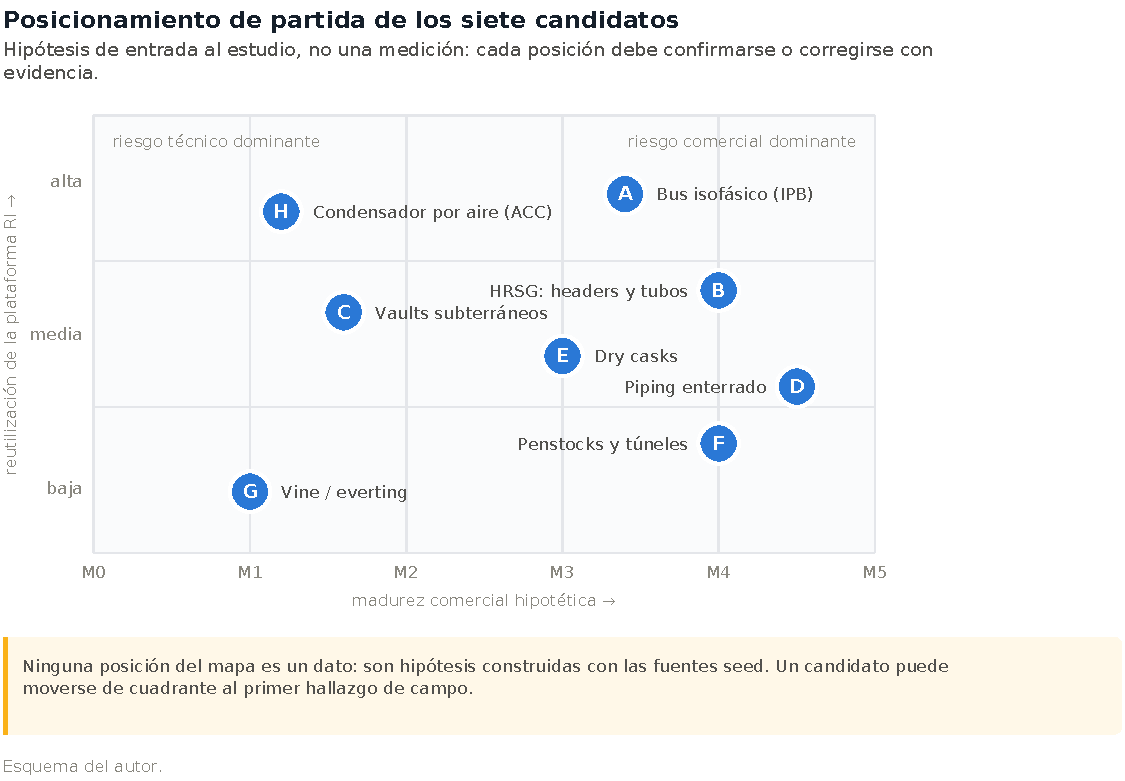
\includegraphics[width=0.98\linewidth]{assets/fig-mapa-candidatos.pdf}}
\caption*{\footnotesize\raggedright Figura 1 — Posicionamiento de partida de los ocho candidatos. {\color{gray2}Elaboración propia sobre las fuentes del Anexo A.}}
\end{figure}

\subsection*{Qué dice hoy la evidencia}
\addcontentsline{toc}{subsection}{Qué dice hoy la evidencia}

\begin{tarjeta}{Donde hay valor probado}{Candidatos A y D}
El valor económico está \textbf{publicado y es alto} en bus isofásico y en piping enterrado: reducción de costo cercana a un orden de magnitud en un caso reportado, y ahorros de entre uno y cinco millones de dólares por utilización, respectivamente. En ambos casos la contrapartida es madurez comercial alta.

\end{tarjeta}
\begin{tarjeta}{Donde hay incumbente}{Candidatos B, D y F}
HRSG, piping enterrado y penstocks tienen proveedor establecido. Entrar exige demostrar un \hyperlink{g-whitespace}{espacio no cubierto (\emph{whitespace})}\textsuperscript{\textsc{g}} concreto —una geometría, un acceso o una medición que el incumbente no cubre—, no una plataforma equivalente.

\end{tarjeta}
\begin{tarjeta}{Donde el problema sigue abierto}{Candidatos C, G y H}
Vaults subterráneos mantiene actividad de investigación vigente con prototipos y demostraciones en curso, sin producto consolidado. Los robots everting son una tecnología sin mercado asignado. En condensadores refrigerados por aire, los propios operadores declaran que la mayor parte del activo \textbf{no se inspecciona} por razones de acceso.

\end{tarjeta}
\begin{notainferencia}{El hallazgo más útil del barrido ampliado}
En seis de las siete familias de activos barridas, el mercado ya está ocupado o el hueco aparente está cerrado por una razón física conocida. La excepción —condensadores refrigerados por aire— no destaca porque la inspección sea cara, sino porque \textbf{hoy no se hace}: es una necesidad declarada por los operadores y no cubierta por los proveedores actuales.

\end{notainferencia}

\subsection*{Qué no debería desarrollarse sin un hallazgo que lo justifique}
\addcontentsline{toc}{subsection}{Qué no debería desarrollarse sin un hallazgo que lo justifique}

\begin{itemize}
\item Un \textbf{\hyperlink{g-crawler}{crawler}\textsuperscript{\textsc{g}} genérico de tuberías}: el problema ya está resuelto comercialmente y el valor lo captura un proveedor establecido.
\item Un \textbf{robot nadador para transformadores} que replique una función ya cubierta por el producto de referencia del mercado.
\item \textbf{Otro cuadrúpedo o vehículo de patrulla} de subestaciones: el valor diferencial está en la carga sensora y la analítica, no en la plataforma.
\item Un \textbf{crawler de línea de transmisión} para inspección visual de rutina, salvo que se demuestre que los drones no lo hicieron económicamente obsoleto.
\end{itemize}


\subsection*{Las incógnitas que bloquean la decisión}
\addcontentsline{toc}{subsection}{Las incógnitas que bloquean la decisión}

\begin{enumerate}
\item Qué parte del problema de HRSG \textbf{no} resuelve hoy el incumbente, con evidencia independiente y no comercial.
\item Cuántos activos direccionables existen por año y a qué ticket real se contrata cada inspección, según contratos y licitaciones y no según informes de mercado.
\item Qué familias de patentes vigentes cubren las arquitecturas candidatas.
\item Qué exige la calificación regulatoria en los candidatos nucleares y cuánto cuesta obtenerla.
\item Si el problema de vaults subterráneos sostiene un ticket recurrente o es un servicio de baja frecuencia y bajo precio.
\item Si en condensadores refrigerados por aire el robot puede evitar el andamiaje, que es donde está la mayor parte del costo, o si igual hay que montarlo para posicionarlo.
\end{enumerate}

\begin{notariesgo}{El error que este estudio existe para evitar}
Descubrir dentro de dos años que el problema ya había sido investigado por una organización de referencia, que un fabricante ya había patentado la arquitectura, que existía un producto comercial establecido, que el cliente ya compraba ese servicio o que hubo un programa de desarrollo que fracasó por una razón física conocida.

\end{notariesgo}
\clearpage

\section*{Parte I — Marco de decisión}
\addcontentsline{toc}{section}{Parte I — Marco de decisión}


\subsection*{1. Objetivo y alcance}
\addcontentsline{toc}{subsection}{1. Objetivo y alcance}


\subsubsection*{1.1 Qué produce este estudio}
\addcontentsline{toc}{subsubsection}{1.1 Qué produce este estudio}

Una recomendación de inversión sostenida por evidencia verificable, que separa con claridad tres cosas distintas:

\begin{enumerate}
\item \textbf{Lo que sabemos}, con fuente y nivel de evidencia declarados.
\item \textbf{Lo que inferimos}, etiquetado como inferencia de ingeniería.
\item \textbf{Lo que todavía debe validarse}, con un plan concreto para hacerlo.
\end{enumerate}

La conclusión debe responder sin ambigüedad: \textbf{¿cuál debería ser el próximo robot que se desarrolle, y por qué?}


\subsubsection*{1.2 Perfiles que requiere el análisis}
\addcontentsline{toc}{subsubsection}{1.2 Perfiles que requiere el análisis}

El estudio combina seis competencias, porque una oportunidad puede caerse por cualquiera de ellas:

\begin{itemize}
\item ingeniería sénior de robótica de inspección;
\item especialidad en \hyperlink{g-nde}{ensayos no destructivos (NDE/NDT)}\textsuperscript{\textsc{g}};
\item análisis de mercado industrial B2B;
\item mantenimiento de generación eléctrica;
\item investigación de \hyperlink{g-prior-art}{\emph{prior art}}\textsuperscript{\textsc{g}} y patentes;
\item análisis de producto y estrategia.
\end{itemize}


\subsubsection*{1.3 Qué queda fuera}
\addcontentsline{toc}{subsubsection}{1.3 Qué queda fuera}

\begin{itemize}
\item No es un diseño de detalle: las propuestas de robot se definen por requisitos funcionales, no por ingeniería de producto.
\item No es una opinión legal de \hyperlink{g-fto}{libertad de operación}\textsuperscript{\textsc{g}}. El análisis de patentes es un \textbf{screening preliminar de propiedad intelectual}.
\item No es un dimensionamiento de mercado basado en informes genéricos de la industria. Cuando no hay datos suficientes para un cálculo defendible, el tamaño de mercado no se publica.
\end{itemize}


\subsection*{2. Qué hace rentable un negocio de robótica de inspección}
\addcontentsline{toc}{subsection}{2. Qué hace rentable un negocio de robótica de inspección}


\subsubsection*{2.1 La lógica del producto de referencia}
\addcontentsline{toc}{subsubsection}{2.1 La lógica del producto de referencia}

Existe un proyecto de robot de inspección (RI) para generadores con rotor instalado. Se usa como \textbf{\hyperlink{g-benchmark}{benchmark}\textsuperscript{\textsc{g}} económico y tecnológico}, no como oportunidad nueva. Su lógica de negocio define el patrón que se busca replicar:

\begin{itemize}
\item activo extremadamente caro;
\item acceso difícil;
\item la inspección convencional puede exigir gran desmontaje, personal especializado o una parada prolongada;
\item el robot reduce \hyperlink{g-outage}{salida de servicio}\textsuperscript{\textsc{g}}, desmontaje y riesgo;
\item el cliente no compra un robot: compra \textbf{información de condición confiable} y ahorro de mantenimiento;
\item el valor del servicio puede superar ampliamente el costo del hardware;
\item la plataforma integra locomoción, cámaras, iluminación, sensado especializado, posicionamiento, \hyperlink{g-tether}{tether}\textsuperscript{\textsc{g}} y comunicaciones, procesamiento y generación automática de informes.
\end{itemize}

\begin{notainferencia}{Consecuencia para la selección de candidatos}
Una oportunidad es comparable al producto de referencia sólo si reproduce la estructura completa del valor: activo caro \textbf{y} acceso difícil \textbf{y} costo convencional alto \textbf{y} decisión de mantenimiento que depende del resultado. Un activo caro con acceso sencillo no sostiene el modelo.

\end{notainferencia}

\subsubsection*{2.2 Restricciones y filosofía de producto}
\addcontentsline{toc}{subsubsection}{2.2 Restricciones y filosofía de producto}

Ocho criterios se aplican a toda solución propuesta, y funcionan como filtro de diseño antes que como preferencia estética.

\begin{tarjeta}{1. Calidad industrial}{}
Hardware apto para servicio profesional repetido y alta confiabilidad. Un prototipo de campo no es un producto de servicio.

\end{tarjeta}
\begin{tarjeta}{2. Costo/beneficio}{}
Se evitan soluciones metrológicas o robóticas innecesariamente exóticas cuando una arquitectura commodity logra el mismo resultado.

\end{tarjeta}
\begin{tarjeta}{3. Componentes commodity}{}
Se prefieren componentes con múltiples fabricantes y cadena de suministro amplia, por disponibilidad y por costo de repuesto.

\end{tarjeta}
\begin{tarjeta}{4. Industrialización}{}
Se evalúa manufacturabilidad, mantenimiento, calibración, reemplazo de consumibles y vida útil desde el primer concepto.

\end{tarjeta}
\begin{tarjeta}{5. Argentina y Latinoamérica}{}
Disponibilidad de componentes, soporte, importación y exportación, y potencial real de mercado regional.

\end{tarjeta}
\begin{tarjeta}{6. Precio real}{}
Se buscan precios efectivos: distribuidores, contratos públicos, licitaciones, integradores o mercado usado. Las estimaciones se etiquetan como tales.

\end{tarjeta}
\begin{tarjeta}{7. Recuperación y \hyperlink{g-fme}{FME}\textsuperscript{\textsc{g}}}{}
En generación eléctrica y nuclear, un robot atrapado puede ser peor que no inspeccionar. La estrategia de recuperación es parte del producto.

\end{tarjeta}
\begin{tarjeta}{8. Servicio antes que hardware}{}
Si la frecuencia por activo es baja pero el ticket por inspección es alto, el modelo de \hyperlink{g-raas}{inspección como servicio}\textsuperscript{\textsc{g}} puede superar a la venta de equipos.

\end{tarjeta}

\subsection*{3. Disciplina de evidencia}
\addcontentsline{toc}{subsection}{3. Disciplina de evidencia}


\subsubsection*{3.1 Cuatro clases de afirmación que nunca deben mezclarse}
\addcontentsline{toc}{subsubsection}{3.1 Cuatro clases de afirmación que nunca deben mezclarse}

\begin{tarjeta}{A \textperiodcentered{} Hecho verificado}{\badge{navy}{white}{A}}
Información respaldada por una fuente primaria o independiente de alta calidad.

\emph{Ejemplo:} EPRI estima ahorros mayores a un millón y menores a cinco millones de dólares por utilización en una aplicación específica de crawler para tuberías enterradas [EPRI MTA-MA-017].

\end{tarjeta}
\begin{tarjeta}{B \textperiodcentered{} Declarado por el fabricante}{\badge{lamber}{amber}{Declaración}}
Afirmación comercial del fabricante o proveedor. \textbf{No se convierte en validación independiente.}

\emph{Ejemplo:} TesTex declara que su herramienta de acceso interno inspecciona todos los tubos conectados a un header en tres o cuatro turnos.

\end{tarjeta}
\begin{tarjeta}{C \textperiodcentered{} Inferencia de ingeniería}{\badge{lamber}{amber}{Inferencia}}
Conclusión razonada del autor a partir de la evidencia disponible. Se etiqueta explícitamente en el texto.

\end{tarjeta}
\begin{tarjeta}{D \textperiodcentered{} Estimación comercial}{\badge{lamber}{amber}{Estimación}}
Cálculo propio de mercado, ticket, ahorro o volumen. Debe mostrar fórmula, supuestos, rango, fuente de cada entrada y sensibilidad. \textbf{Nunca se presenta como dato publicado.}

\end{tarjeta}

\subsubsection*{3.2 Jerarquía de fuentes}
\addcontentsline{toc}{subsubsection}{3.2 Jerarquía de fuentes}

\begin{figure}[htbp]\centering
\fbox{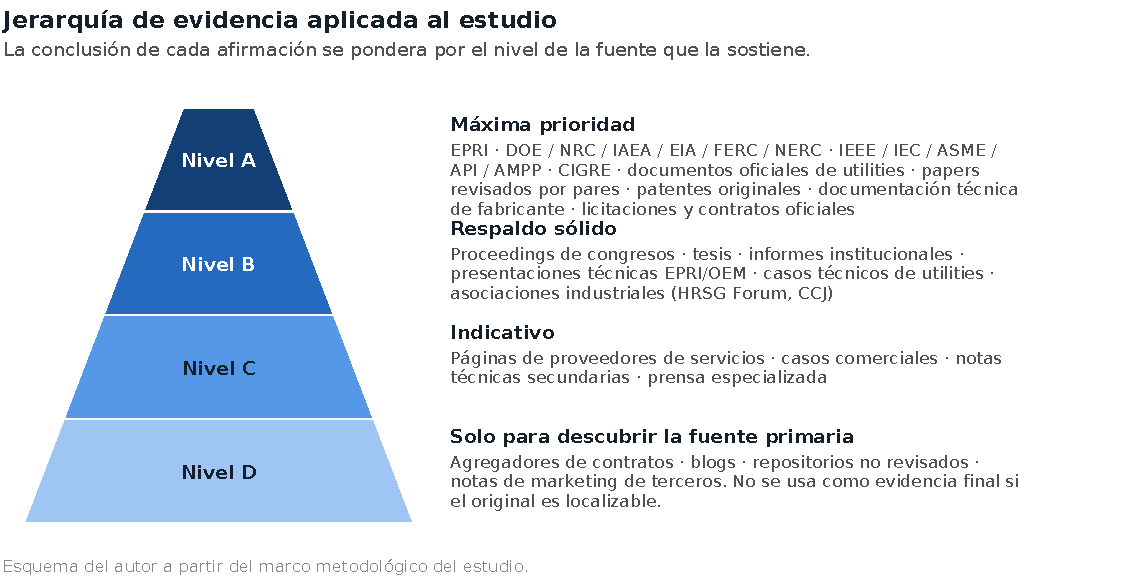
\includegraphics[width=0.98\linewidth]{assets/fig-evidencia.pdf}}
\caption*{\footnotesize\raggedright Figura 2 — Jerarquía de evidencia y familias de fuentes de cada nivel. {\color{gray2}Elaboración propia.}}
\end{figure}
El nivel D sirve únicamente para \textbf{descubrir} la fuente primaria. No se usa como evidencia final si el original puede localizarse.


\subsubsection*{3.3 Diez reglas de verificación}
\addcontentsline{toc}{subsubsection}{3.3 Diez reglas de verificación}

\begin{enumerate}
\item \textbf{Una patente demuestra divulgación, no funcionamiento comercial.} Se verifica familia, titular, prioridad, estado legal y expiración o abandono cuando sea relevante.
\item \textbf{Un prototipo universitario no es un producto.}
\item \textbf{Un producto anunciado no equivale a despliegue de campo.} Se buscan clientes, sitios, fechas, cantidad de inspecciones y evidencia de repetición.
\item \textbf{Una reducción de costos publicada por el fabricante se identifica como tal}, no como resultado independiente.
\item \textbf{No se usan informes de mercado opacos} del tipo «mercado de X mil millones de dólares» como base principal.
\item Si no existe precio publicado: se escribe \emph{precio no publicado} y se buscan contratos, licitaciones y distribuidores. No se inventa.
\item Si no hay evidencia de competencia: se escribe \emph{no se identificó competencia después de las búsquedas X, Y y Z}. No se escribe \emph{no existe competencia}.
\item Se buscan productos \textbf{actuales, discontinuados, adquiridos y fallidos}.
\item Se busca en inglés y, cuando corresponda, también en alemán, japonés, chino, coreano, francés, español y portugués: empresas relevantes pueden no estar bien indexadas en inglés.
\item Cada candidato recibe, como mínimo, búsquedas por activo en la base del instituto de investigación sectorial; búsquedas por robótica, inspección remota y automatización; búsqueda web general; búsqueda de patentes en las bases internacionales; revisión de fabricantes y de utilities; literatura técnica revisada; licitaciones y contratos; y material audiovisual técnico sólo como evidencia suplementaria.
\end{enumerate}


\subsubsection*{3.4 Escala de madurez comercial}
\addcontentsline{toc}{subsubsection}{3.4 Escala de madurez comercial}

\begin{figure}[htbp]\centering
\fbox{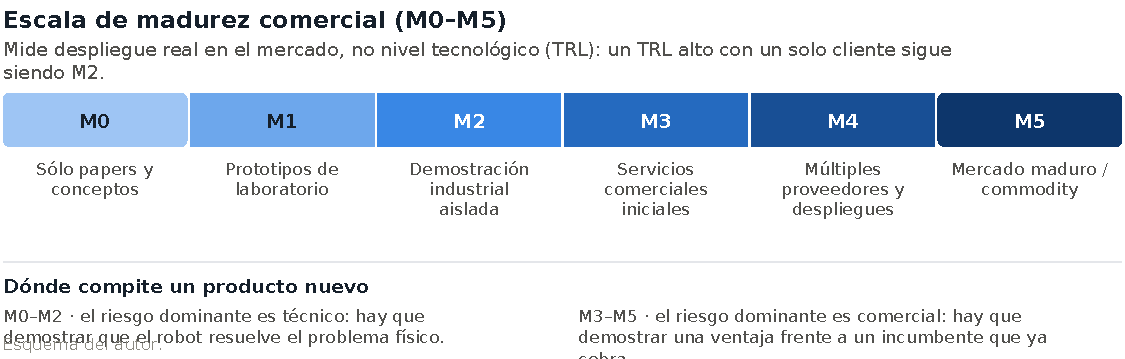
\includegraphics[width=0.98\linewidth]{assets/fig-madurez.pdf}}
\caption*{\footnotesize\raggedright Figura 3 — Escala de madurez comercial M0–M5 usada en todo el documento. {\color{gray2}Elaboración propia.}}
\end{figure}
\begin{notariesgo}{No confundir madurez con nivel tecnológico}
Un desarrollo puede tener \hyperlink{g-trl}{nivel tecnológico}\textsuperscript{\textsc{g}} alto y madurez comercial baja: la escala mide \textbf{despliegue real en el mercado}, no capacidad demostrada en laboratorio.

\end{notariesgo}

\subsection*{4. Proceso de evaluación}
\addcontentsline{toc}{subsection}{4. Proceso de evaluación}

\begin{figure}[htbp]\centering
\fbox{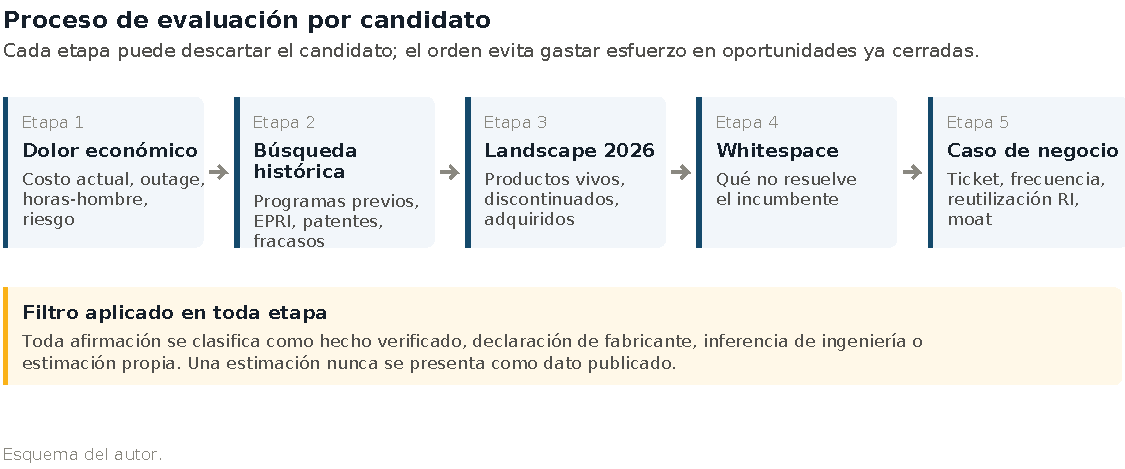
\includegraphics[width=0.98\linewidth]{assets/fig-proceso.pdf}}
\caption*{\footnotesize\raggedright Figura 4 — Secuencia de evaluación por candidato y filtro de clasificación de evidencia. {\color{gray2}Elaboración propia.}}
\end{figure}

\subsubsection*{4.1 La búsqueda histórica es obligatoria}
\addcontentsline{toc}{subsubsection}{4.1 La búsqueda histórica es obligatoria}

Para cada candidato se reconstruye una línea temporal completa, además de la búsqueda del estado actual.

\begin{figure}[htbp]\centering
\fbox{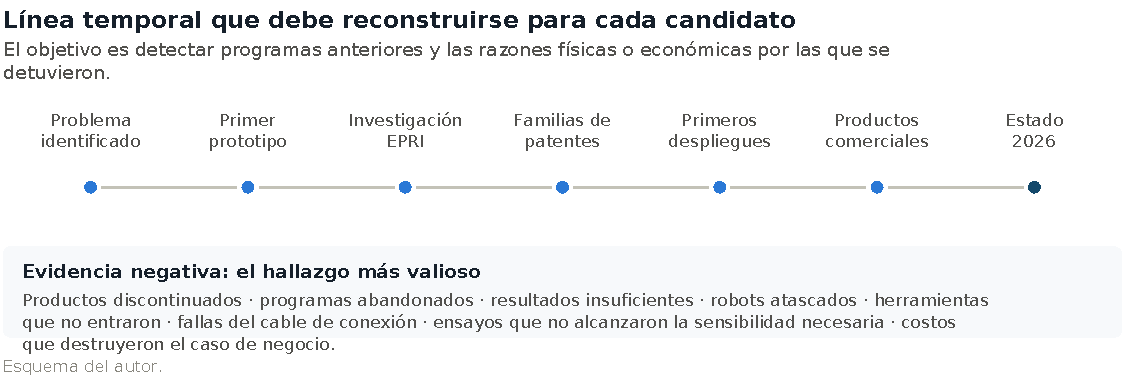
\includegraphics[width=0.98\linewidth]{assets/fig-cronologia.pdf}}
\caption*{\footnotesize\raggedright Figura 5 — Línea temporal de prior art que debe reconstruirse por candidato. {\color{gray2}Elaboración propia.}}
\end{figure}

\subsubsection*{4.2 Las fuentes negativas son las más valiosas}
\addcontentsline{toc}{subsubsection}{4.2 Las fuentes negativas son las más valiosas}

Un programa que se detuvo explica más que diez folletos comerciales. Se documentan explícitamente:

\begin{itemize}
\item productos discontinuados y programas abandonados;
\item resultados insuficientes publicados en literatura técnica;
\item robots que quedaron atascados y herramientas que no entraron;
\item eventos de material extraño (FME) y fallas de tether;
\item ensayos no destructivos que no alcanzaron la sensibilidad requerida;
\item costos que destruyeron el \hyperlink{g-caso-negocio}{caso de negocio}\textsuperscript{\textsc{g}}.
\end{itemize}

\clearpage

\section*{Parte II — Mapa de oportunidades}
\addcontentsline{toc}{section}{Parte II — Mapa de oportunidades}


\subsection*{5. Panorama y criterio de entrada}
\addcontentsline{toc}{subsection}{5. Panorama y criterio de entrada}

Los ocho candidatos que siguen no son una conclusión: son el punto de partida verificado hasta la fecha de corte. \textbf{Ninguno se da por válido}: cada uno se verifica desde cero y se descarta si la evidencia lo exige. Si durante la verificación aparece que un candidato está saturado, que el incumbente cerró el hueco o que otra aplicación ofrece un negocio mejor, el orden cambia.

Cada ficha responde siempre a la misma estructura: geometría y problema, hipótesis de valor, evidencia disponible con su nivel, competencia identificada, pregunta estratégica que decide el caso y agenda de verificación pendiente.


\subsection*{6. Candidato A — Bus isofásico (IPB)}
\addcontentsline{toc}{subsection}{6. Candidato A — Bus isofásico (IPB)}

\begin{figure}[htbp]\centering
\fbox{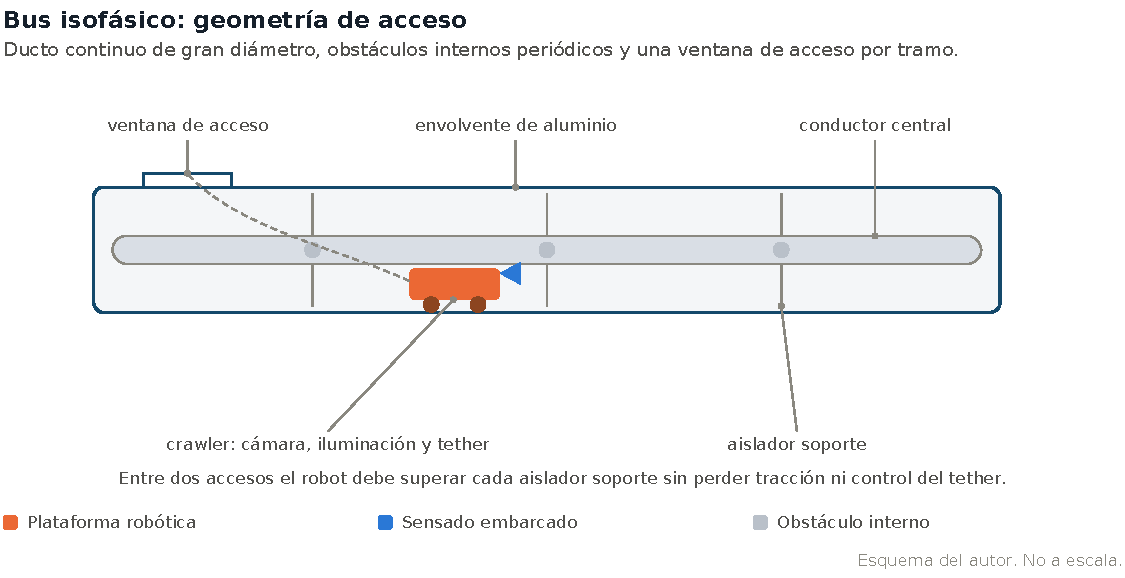
\includegraphics[width=0.98\linewidth]{assets/esq-ipb.pdf}}
\caption*{\footnotesize\raggedright Figura 6 — Geometría de acceso del bus isofásico y obstáculos internos. {\color{gray2}Esquema del autor.}}
\end{figure}

\subsubsection*{6.1 Hipótesis de valor}
\addcontentsline{toc}{subsubsection}{6.1 Hipótesis de valor}

Puede ser la extensión inmediata más natural del producto de referencia:

\begin{itemize}
\item mismo tipo de cliente;
\item inspección durante paradas programadas;
\item espacio confinado;
\item reducción de andamiaje y de entrada de personal;
\item alta reutilización de cámaras, tether, iluminación, software de mapeo y arquitectura de crawler.
\end{itemize}


\subsubsection*{6.2 Evidencia disponible}
\addcontentsline{toc}{subsubsection}{6.2 Evidencia disponible}

\begin{notadato}{Dato EPRI verificado — MTA-MA-029 \badge{navy}{white}{A}}
Experiencia reportada por una utility con costo de proveedor de aproximadamente \textbf{USD 100.000 por implementación}; ejecución de la inspección en \textbf{menos de un día}; reducción de costo de aproximadamente \textbf{10$\times$} frente a la inspección manual en ese caso; \hyperlink{g-payback}{payback}\textsuperscript{\textsc{g}} inmediato según la evaluación \hyperlink{g-sweep}{SWEEP}\textsuperscript{\textsc{g}}; tecnología comercialmente disponible; riesgos identificados de falla de crawler o de herramienta. Una parte sustancial del ahorro proviene de evitar andamiaje y acceso humano.

\textbf{Este dato no se generaliza al mercado completo sin evidencia adicional.}

\end{notadato}
\begin{figure}[htbp]\centering
\fbox{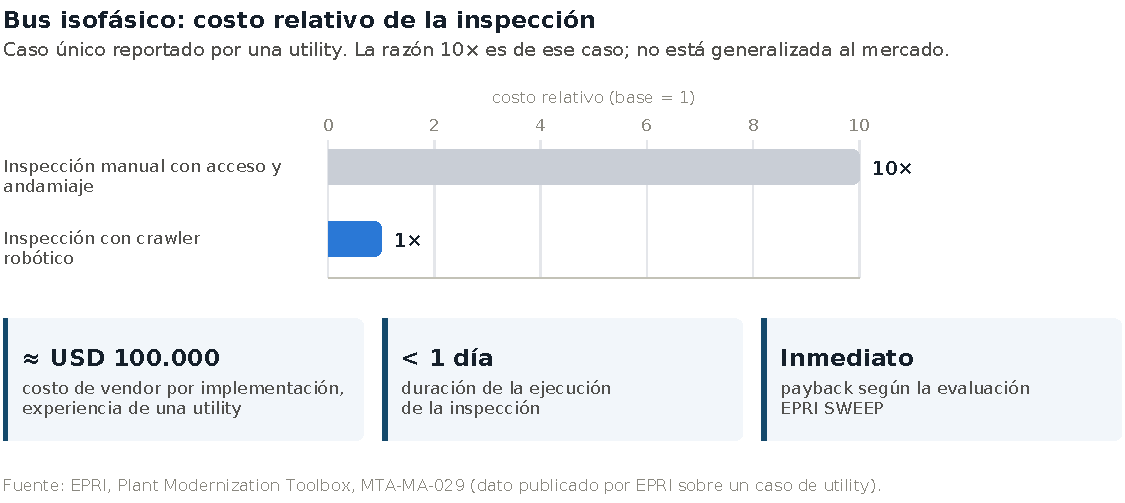
\includegraphics[width=0.98\linewidth]{assets/fig-ipb-economia.pdf}}
\caption*{\footnotesize\raggedright Figura 7 — Costo relativo de la inspección de bus isofásico e indicadores del caso reportado. {\color{gray2}EPRI, Plant Modernization Toolbox, MTA-MA-029.}}
\end{figure}
\begin{notariesgo}{Advertencia de recurrencia, verificada en fuente primaria \badge{navy}{white}{A}}
EPRI declara que las inspecciones de bus isofásico se realizan \textbf{típicamente cada 10 años}. El candidato A combina entonces valor alto por intervención con recurrencia baja: un activo que se inspecciona una vez por década sólo sostiene un negocio de servicio si la base instalada accesible es grande.

El criterio de recurrencia del Ranking A penaliza a este candidato más de lo que suponía la hipótesis de partida, y el dimensionamiento debe hacerse sobre inspecciones por año, no sobre cantidad de activos.

\emph{Nota de calidad de fuente:} en ese mismo documento, la tabla del bus isofásico repite literalmente la frase de horas-hombre de la tabla de estructuras de toma de agua, incluida la explicación de que el rango depende de la calidad del agua, que no aplica a un ducto de barras. Por esa inconsistencia \textbf{no se utiliza} ninguna cifra de horas-hombre para este candidato desde esa fuente.

\end{notariesgo}
De la guía de mantenimiento de bus aislado por fases (EPRI 1015057) deben extraerse: frecuencia típica de inspección, modos de defecto, condiciones de acceso, figuras de plataformas robóticas existentes, mantenimiento recomendado y mediciones eléctricas asociadas.


\subsubsection*{6.3 Competencia identificada para verificación}
\addcontentsline{toc}{subsubsection}{6.3 Competencia identificada para verificación}

Trident NGS \textperiodcentered{} Electrical Builders Inc. \textperiodcentered{} MidStates Energy \textperiodcentered{} nVent \textperiodcentered{} áreas de servicio de GE Vernova, Siemens Energy e Hitachi Energy \textperiodcentered{} empresas especializadas del sector nuclear \textperiodcentered{} sistemas de origen coreano, japonés y chino \textperiodcentered{} desarrollos universitarios, entre ellos los de la Universidad de Beihang.

La evolución posible del alcance —de cámara sobre crawler a limpieza, retiro de material extraño, verificación de torque, medición de resistencia y manipulación— debe evaluarse contra el catálogo de tareas de alto valor de EPRI 3002023899.

De cada uno debe registrarse: nombre exacto del equipo, fabricante, tipo de locomoción, dimensiones, tether o inalámbrico, forma de superar aisladores y soportes, estrategia de recuperación, sensores, capacidad de limpieza, medición de torque o resistencia, precio del servicio, clientes y frecuencia de inspección.

\begin{notaclave}{Pregunta estratégica que decide el candidato}
¿Existe espacio para un sistema de \textbf{inspección y mantenimiento} —limpieza, retiro de material extraño, verificación de torque, medición de resistencia, manipulación— y no solamente para otro crawler con cámara?

\end{notaclave}
\begin{detalle}{Agenda de verificación pendiente}
\begin{itemize}
\item Confirmar si el valor de USD 100.000 corresponde a un contrato típico o a un caso aislado, contrastando con licitaciones y contratos de utilities.
\item Determinar la frecuencia real de inspección por tramo y por central.
\item Establecer si el ahorro por evitar andamiaje se sostiene en plantas con accesos ya construidos.
\item Verificar el estado 2026 de cada proveedor identificado: activo, discontinuado, adquirido o sin comercialización.
\item Buscar patentes sobre crawlers para ductos de barras y sobre mecanismos de superación de aisladores.
\end{itemize}

\end{detalle}

\subsection*{7. Candidato B — HRSG: headers, soldaduras y tubos}
\addcontentsline{toc}{subsection}{7. Candidato B — HRSG: headers, soldaduras y tubos}

\begin{figure}[htbp]\centering
\fbox{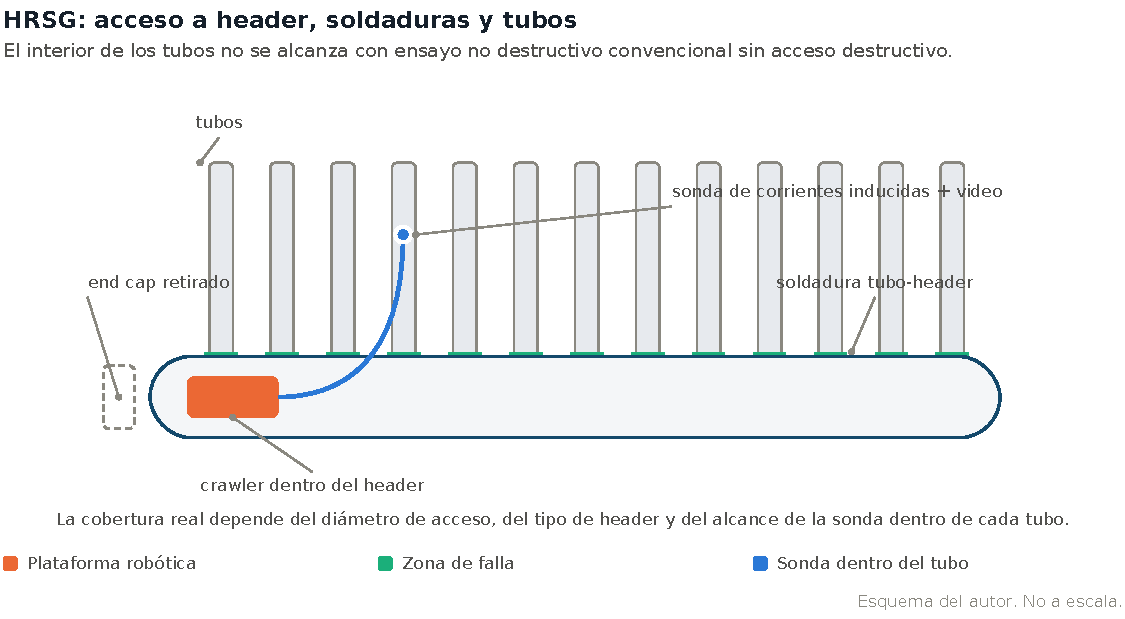
\includegraphics[width=0.98\linewidth]{assets/esq-hrsg.pdf}}
\caption*{\footnotesize\raggedright Figura 8 — Acceso a header, soldaduras tubo-header y tubos en una caldera de recuperación. {\color{gray2}Esquema del autor.}}
\end{figure}

\subsubsection*{7.1 El problema físico}
\addcontentsline{toc}{subsubsection}{7.1 El problema físico}

El estudio EPRI 1017635 sobre tecnología de robots tipo serpiente para inspección de \hyperlink{g-header}{headers}\textsuperscript{\textsc{g}} y tubos en calderas de recuperación de calor documenta el punto de partida: ciertos tubos interiores \textbf{no pueden inspeccionarse fácilmente con ensayos no destructivos convencionales sin acceso destructivo}. De ese informe deben extraerse las razones por las que la inspección convencional no llega, las geometrías y diámetros involucrados, las longitudes, los tipos de caldera, los puntos de acceso, las modalidades de inspección evaluadas, los conceptos de robot analizados, lo que se demostró, lo que quedó sin resolver y por qué ese concepto no se comercializó directamente.


\subsubsection*{7.2 El incumbente}
\addcontentsline{toc}{subsubsection}{7.2 El incumbente}

\begin{notadato}{Declarado por el fabricante — TesTex \badge{lamber}{amber}{Declaración}}
La herramienta de acceso interno (IAT) es un crawler que se coloca dentro del header; puede ingresar por la tapa del extremo o, en versión modular, por un orificio de aproximadamente 8 pulgadas; empuja una sonda de \hyperlink{g-rfet}{corrientes inducidas por campo remoto}\textsuperscript{\textsc{g}} junto con una cámara a lo largo de los tubos; se opera en forma remota; según el fabricante inspecciona todos los tubos de un header en tres o cuatro turnos y declara cobertura del 100 \% de los tubos dentro de sus condiciones de aplicación, con despliegues en múltiples utilities.

La herramienta complementaria de inspección de soldaduras por campo lejano declara del orden de 200 soldaduras por turno.

\textbf{Ninguna de estas cifras es evidencia independiente hasta que se contraste con clientes, contratos o literatura técnica.}

\end{notadato}

\subsubsection*{7.3 Competencia y fuentes adicionales a recorrer}
\addcontentsline{toc}{subsubsection}{7.3 Competencia y fuentes adicionales a recorrer}

Patentes de TesTex \textperiodcentered{} desarrollos conjuntos entre EPRI y TesTex \textperiodcentered{} \emph{Combined Cycle Journal} y el HRSG Forum \textperiodcentered{} fabricantes de calderas de recuperación: Nooter/Eriksen, Vogt, Alstom/Altrad \textperiodcentered{} GE Vernova \textperiodcentered{} Siemens Energy \textperiodcentered{} EDF \textperiodcentered{} proveedores de servicios de ensayos no destructivos: MISTRAS \textperiodcentered{} fabricantes de instrumentación: Eddyfi, Waygate/Baker Hughes, Olympus/Evident \textperiodcentered{} robots académicos para tubos de caldera \textperiodcentered{} crawlers magnéticos \textperiodcentered{} robots serpiente y robots continuos.

\begin{notaclave}{Pregunta estratégica que decide el candidato}
El mercado no está vacío. La pregunta correcta es: \textbf{¿qué parte del problema no resuelve hoy el incumbente?}

Hipótesis a validar: menor diámetro de acceso; no retirar la tapa del extremo; más tipos de header cubiertos; indexado automático de tubos; mayor alcance dentro del tubo; mejor localización; un solo despliegue que cubra soldadura y espesor de pared; medición cuantitativa superior; mayor autonomía; capacidad frente a depósitos y bloqueos; inspección combinada con limpieza o reparación.

Si no aparece un hueco defendible, el candidato baja en el ranking.

\end{notaclave}
\begin{detalle}{Agenda de verificación pendiente}
\begin{itemize}
\item Obtener evidencia independiente de cobertura real por header y por turno.
\item Determinar qué proporción del parque de calderas queda fuera del alcance del incumbente por geometría.
\item Cuantificar el costo de una parada por falla de soldadura tubo-header frente al costo de la inspección.
\item Revisar la familia de patentes del incumbente y su estado legal.
\end{itemize}

\end{detalle}

\subsection*{8. Candidato C — Vaults subterráneos de transmisión}
\addcontentsline{toc}{subsection}{8. Candidato C — Vaults subterráneos de transmisión}

\begin{figure}[htbp]\centering
\fbox{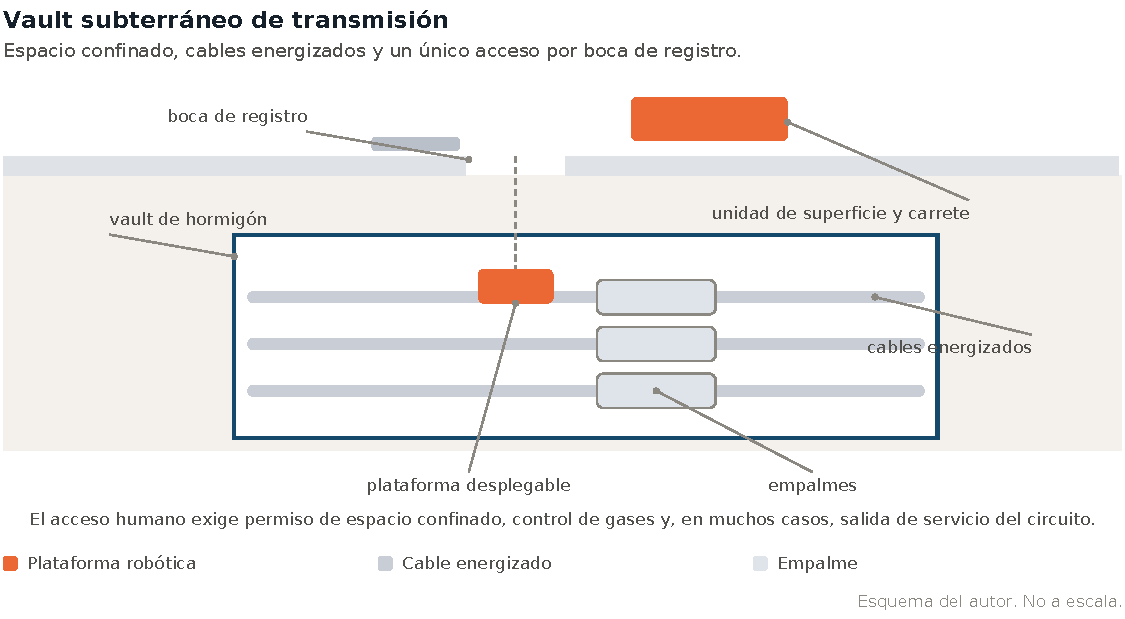
\includegraphics[width=0.98\linewidth]{assets/esq-vault.pdf}}
\caption*{\footnotesize\raggedright Figura 9 — Vault subterráneo con cables energizados, empalmes y acceso por boca de registro. {\color{gray2}Esquema del autor.}}
\end{figure}

\subsubsection*{8.1 Estado de la investigación}
\addcontentsline{toc}{subsubsection}{8.1 Estado de la investigación}

\begin{notadato}{Investigación vigente \badge{navy}{white}{A}}
El programa de transmisión subterránea de EPRI publicó \emph{Underground Transmission Vault Inspection Using Robotic Techniques} (3002000878) sobre inspección de \hyperlink{g-vault}{vaults}\textsuperscript{\textsc{g}} en 2013 y mantiene el trabajo con la actualización 2025 (3002032834) y actividad declarada para 2026 y 2027. Los objetivos declarados son mejorar la seguridad de los trabajadores y reducir los requerimientos de salida de servicio del circuito. Se reportan conceptos y prototipos demostrados en laboratorio y en sitios de utilities, con demostraciones en planificación.

\end{notadato}
Existe además un proyecto complementario sobre inspección de bocas de registro con cable extruido dentro de los proyectos suplementarios colaborativos 2025–2026, cuya arquitectura debe caracterizarse: inspección desde la superficie, cable energizado, termografía infrarroja, cámara, detección de gases, brazo mecánico y, si aplica, descargas parciales o medición acústica y ultrasónica.


\subsubsection*{8.2 Competencia a investigar}
\addcontentsline{toc}{subsubsection}{8.2 Competencia a investigar}

Osmose \textperiodcentered{} utilities con desarrollo propio: Con Edison, National Grid, Southern California Edison, PG\&E, NYPA, Duke Energy, Dominion, Entergy e Hydro-Québec \textperiodcentered{} empresas de crawlers para colectores adaptados \textperiodcentered{} drones de espacio confinado \textperiodcentered{} plataformas cuadrúpedas (Boston Dynamics, ANYbotics) aplicadas a vaults \textperiodcentered{} integradores.

\begin{notaclave}{Pregunta estratégica que decide el candidato}
Este candidato puede estar \textbf{menos maduro} que el bus isofásico o el piping enterrado, lo que es simultáneamente su oportunidad y su riesgo. Debe determinarse: cantidad de vaults, frecuencia de inspección, necesidad de desenergización, costo actual, carga de seguridad y espacio confinado, si puede venderse como servicio recurrente, ticket razonable y requisitos de aislamiento eléctrico y detección de gases.

\end{notaclave}
\begin{detalle}{Agenda de verificación pendiente}
\begin{itemize}
\item Contactar a los responsables técnicos del programa de transmisión subterránea de EPRI —David Kummer, inspección robótica, y Tom Zhao, dirección del programa— verificando previamente que sigan en esos roles.
\item Buscar el proyecto \emph{Extruded Cable Manhole Inspections} dentro de los proyectos suplementarios colaborativos 2025–2026.
\item Obtener el censo de vaults de al menos dos utilities y su plan de inspección.
\item Verificar si la inspección hoy exige salida de servicio y cuánto cuesta esa salida.
\item Determinar si el comprador es el área de mantenimiento, la de seguridad o la de ingeniería de activos.
\end{itemize}

\end{detalle}

\subsection*{9. Candidato D — Piping enterrado e inaccesible}
\addcontentsline{toc}{subsection}{9. Candidato D — Piping enterrado e inaccesible}

\begin{figure}[htbp]\centering
\fbox{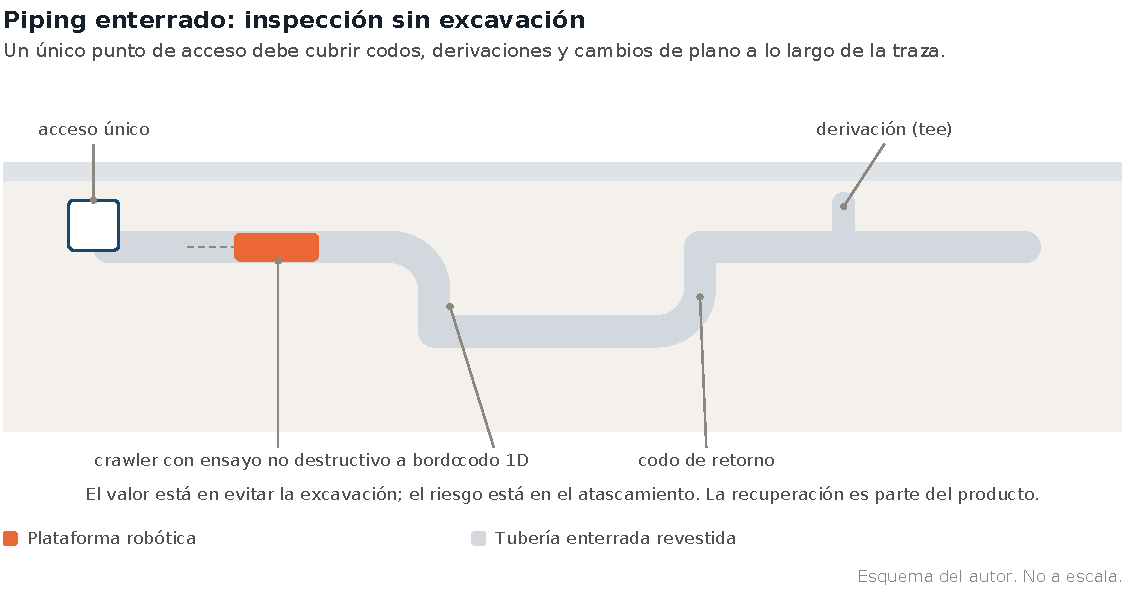
\includegraphics[width=0.98\linewidth]{assets/esq-piping.pdf}}
\caption*{\footnotesize\raggedright Figura 10 — Inspección de tubería enterrada desde un acceso único, sin excavación. {\color{gray2}Esquema del autor.}}
\end{figure}

\subsubsection*{9.1 Evidencia disponible}
\addcontentsline{toc}{subsubsection}{9.1 Evidencia disponible}

\begin{notadato}{Dato EPRI verificado — MTA-MA-017 \badge{navy}{white}{A}}
Inspección desde un único punto de acceso, que puede evitar la excavación. La \hyperlink{g-emat}{técnica electromagnética acústica (EMAT)}\textsuperscript{\textsc{g}} permite determinados exámenes volumétricos sin remover el revestimiento. Según la evaluación SWEEP: costo de implementación menor a un millón de dólares; ahorro mayor a un millón y menor a cinco millones por utilización; payback inmediato o menor a un año; tecnología ya comercialmente implementada en el sector nuclear.

\end{notadato}
\begin{figure}[htbp]\centering
\fbox{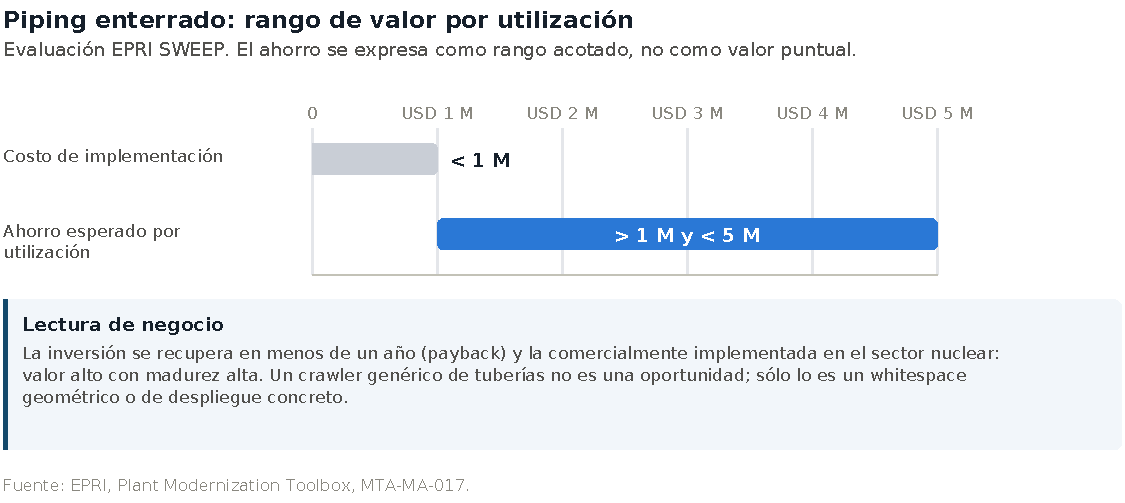
\includegraphics[width=0.98\linewidth]{assets/fig-piping-economia.pdf}}
\caption*{\footnotesize\raggedright Figura 11 — Costo de implementación y rango de ahorro esperado por utilización. {\color{gray2}EPRI, Plant Modernization Toolbox, MTA-MA-017.}}
\end{figure}
De la compilación de lecciones aprendidas sobre tuberías enterradas y subterráneas (EPRI 1025272) deben extraerse: por qué la \hyperlink{g-ili}{inspección en línea}\textsuperscript{\textsc{g}} convencional no funciona bien en instalaciones nucleares, ausencia de estaciones de lanzamiento y recepción, codos, derivaciones, tramos verticales, revestimientos, diámetros, condición con y sin agua, y los eventos de material extraño y recuperación.


\subsubsection*{9.2 Competencia}
\addcontentsline{toc}{subsubsection}{9.2 Competencia}

Diakont, con caso documentado de primera inspección en línea de tubería enterrada en el sector nuclear \textperiodcentered{} Structural Integrity Associates \textperiodcentered{} Westinghouse \textperiodcentered{} Framatome \textperiodcentered{} Eddyfi/Inuktun, incluida la familia VersaTrax \textperiodcentered{} Waygate Technologies \textperiodcentered{} Gecko Robotics \textperiodcentered{} MISTRAS \textperiodcentered{} ROSEN y NDT Global en inspección en línea de hidrocarburos \textperiodcentered{} empresas de inspección de tuberías industriales.

\begin{notaclave}{Pregunta estratégica que decide el candidato}
La evidencia clasifica este candidato como \textbf{comercialmente implementado}. Por lo tanto, \textbf{no debe recomendarse un crawler genérico de tuberías}. Sólo se recomienda si se identifica un hueco concreto: diámetro pequeño, codos de radio corto, derivaciones, reducciones, tramos verticales, transición seco-húmedo, tubería protegida o revestida, inspección combinada con reparación, despliegue sin corte, acceso menor, o un servicio de bajo costo fuera del ámbito nuclear.

\end{notaclave}
\begin{detalle}{Agenda de verificación pendiente}
\begin{itemize}
\item Mapear qué geometrías quedan explícitamente fuera del alcance de los proveedores actuales.
\item Obtener precios de servicio por metro inspeccionado en al menos dos mercados.
\item Evaluar el mercado no nuclear —industrial, municipal, petroquímico— donde el costo de calificación es menor.
\end{itemize}

\end{detalle}

\subsection*{10. Candidato E — Contenedores de combustible gastado en seco}
\addcontentsline{toc}{subsection}{10. Candidato E — Contenedores de combustible gastado en seco}

\begin{figure}[htbp]\centering
\fbox{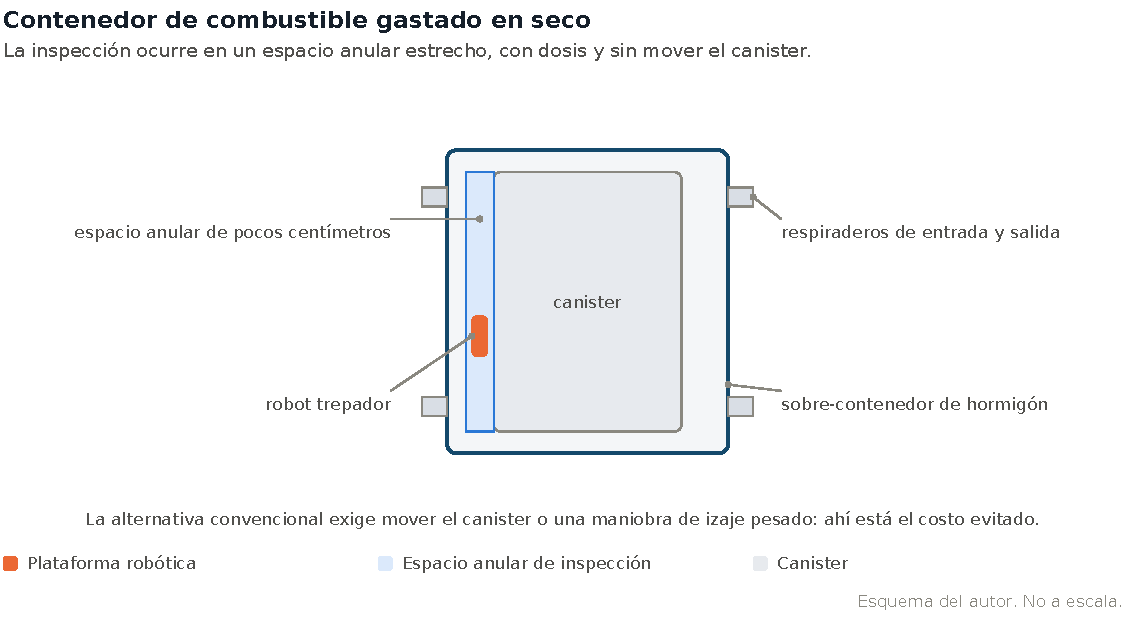
\includegraphics[width=0.98\linewidth]{assets/esq-cask.pdf}}
\caption*{\footnotesize\raggedright Figura 12 — Espacio anular de inspección en un contenedor de almacenamiento en seco. {\color{gray2}Esquema del autor.}}
\end{figure}

\subsubsection*{10.1 Evidencia disponible}
\addcontentsline{toc}{subsubsection}{10.1 Evidencia disponible}

EPRI desarrolla sistemas de inspección y de entrega robótica para almacenamiento en \hyperlink{g-canister}{canister}\textsuperscript{\textsc{g}} seco (3002008234, \emph{Dry Canister Storage System Inspection and Robotic Delivery System Development}), con difusión adicional en EPRI Journal sobre robots trepadores para contenedores. Los elementos verificados hasta la fecha: espacios anulares muy estrechos; combinación de cámara, \hyperlink{g-eca}{corrientes inducidas}\textsuperscript{\textsc{g}}, técnica electromagnética acústica y medición de dosis y temperatura en ciertas configuraciones; múltiples ensayos de campo; y una reducción de costo muy alta frente a los métodos que exigen izaje pesado o movimiento del canister.


\subsubsection*{10.2 Competencia}
\addcontentsline{toc}{subsubsection}{10.2 Competencia}

Robotic Technologies of Tennessee declara que instalaciones nucleares utilizan sus plataformas para inspección de almacenamiento en seco. Deben verificarse: los modelos exactos; los programas de EPRI y del Departamento de Energía; el caso de San Onofre (SONGS); los fabricantes de sistemas de almacenamiento —Holtec, Orano, NAC—; los requisitos de la Comisión Reguladora Nuclear; los desarrollos universitarios asociados, entre ellos los de Penn State y la iniciativa PRINSE; la calificación frente a radiación; y el panorama de patentes.

\begin{notaclave}{Pregunta estratégica que decide el candidato}
El valor por inspección es alto, pero el mercado es limitado, la calificación es exigente, el riesgo de material extraño es crítico, hay dosis y existe un incumbente. Debe compararse rigurosamente contra oportunidades menos reguladas antes de asignarle prioridad.

\end{notaclave}

\subsection*{11. Candidato F — Penstocks y túneles hidroeléctricos}
\addcontentsline{toc}{subsection}{11. Candidato F — Penstocks y túneles hidroeléctricos}

\begin{figure}[htbp]\centering
\fbox{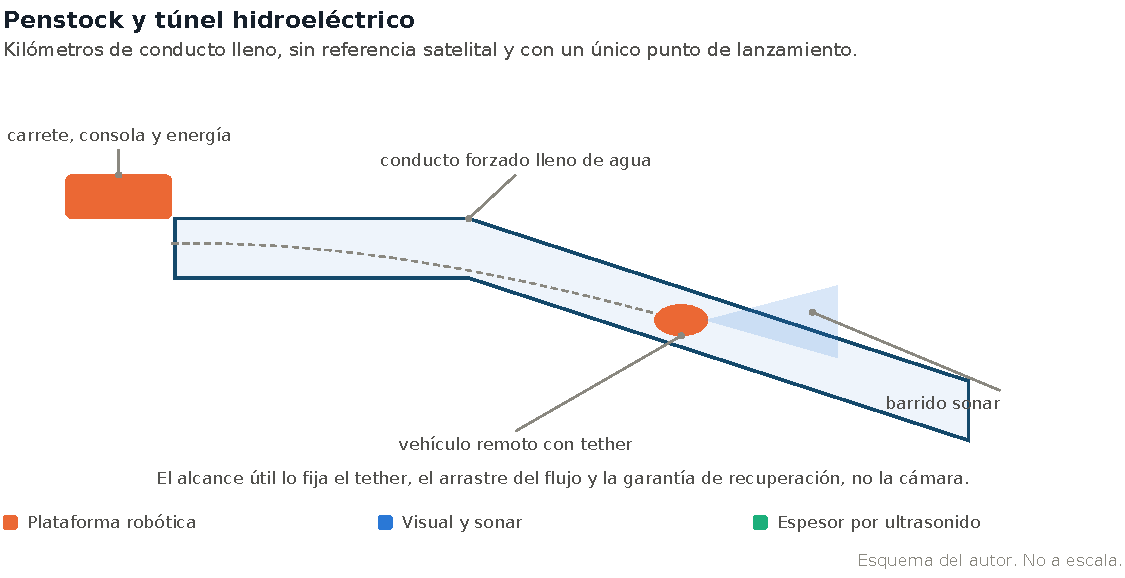
\includegraphics[width=0.98\linewidth]{assets/esq-penstock.pdf}}
\caption*{\footnotesize\raggedright Figura 13 — Inspección de conducto forzado con vehículo remoto y tether. {\color{gray2}Esquema del autor.}}
\end{figure}

\subsubsection*{11.1 Base de evidencia}
\addcontentsline{toc}{subsubsection}{11.1 Base de evidencia}

El informe EPRI sobre tecnología de \hyperlink{g-rov}{vehículos operados remotamente}\textsuperscript{\textsc{g}} en instalaciones hidroeléctricas (TR-113584-V7 / 1007576) aporta: aplicaciones en túnel y \hyperlink{g-penstock}{conducto forzado}\textsuperscript{\textsc{g}}, inspección visual, sonar, medición de espesor por ultrasonido, limitaciones de tether, alcance, recuperación, casos de estudio y ahorro por evitar vaciado y salida de servicio. Debe complementarse con EPRI 3002011682, \emph{Autonomous Underwater Vehicles for Tunnel and Penstock Inspection}, y con la actividad vigente del EPRI Unmanned Mobile Technologies Collaboration Group.


\subsubsection*{11.2 Competencia}
\addcontentsline{toc}{subsubsection}{11.2 Competencia}

Deep Trekker \textperiodcentered{} VideoRay \textperiodcentered{} Eddyfi/Inuktun \textperiodcentered{} Deep Ocean Engineering \textperiodcentered{} Saab Seaeye \textperiodcentered{} integradores sobre plataformas Blue Robotics \textperiodcentered{} vehículos propios de utilities como Hydro-Québec \textperiodcentered{} fabricantes de turbinas con área de servicio: Voith, Andritz y GE Vernova Hydro \textperiodcentered{} proveedores especializados en inspección de túneles.

\begin{notaclave}{Pregunta estratégica que decide el candidato}
La inspección visual con vehículo remoto es probablemente madura. El hueco, si existe, está en: navegación autónoma en distancias kilométricas; localización sin señal satelital; mapeo de espesor de pared; ensayos no destructivos en contacto; recuperación garantizada; operación con turbidez, con caudal alto y con tether largo.

\end{notaclave}

\subsection*{12. Candidato G — Robots everting (vine) para equipos de planta}
\addcontentsline{toc}{subsection}{12. Candidato G — Robots everting (vine) para equipos de planta}

\begin{figure}[htbp]\centering
\fbox{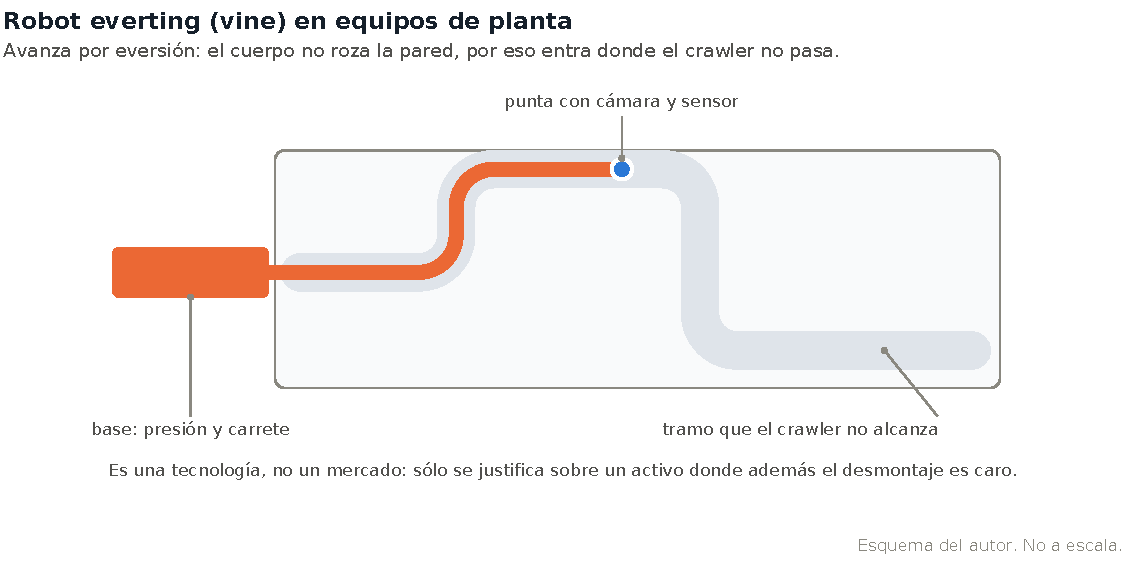
\includegraphics[width=0.98\linewidth]{assets/esq-vine.pdf}}
\caption*{\footnotesize\raggedright Figura 14 — Avance por eversión en un conducto ramificado de equipo de planta. {\color{gray2}Esquema del autor.}}
\end{figure}

\subsubsection*{12.1 Estado}
\addcontentsline{toc}{subsubsection}{12.1 Estado}

EPRI registra sobre \hyperlink{g-vine}{robots everting}\textsuperscript{\textsc{g}} el estudio 3002032954, \emph{Everting Vine Robots for Plant Equipment Inspection – Technology Review and Feasibility Study}, cuyos resultados deben verificarse directamente y sin asumir contenidos no públicos. Como fuentes externas iniciales: la literatura de \emph{IEEE Robotics \& Automation Magazine} sobre robots vine de gran escala para inspección industrial; el trabajo conjunto de UCSB y Bechtel; los desarrollos de Stanford; y las empresas emergentes Trellis Robotics e IvySpec.

\begin{notaclave}{Pregunta estratégica que decide el candidato}
Un robot everting es \textbf{una tecnología, no un mercado}. Sólo se justifica si se identifica un activo concreto donde el crawler no pasa, el boroscopio no alcanza, el desmontaje es costoso y el robot puede transportar un ensayo no destructivo útil.

Candidatos de activo a evaluar: conductos de aire y gases; calderas de recuperación; tramos de tubería compleja; espacios internos de turbina y caldera; conductos de cables; equipos confinados.

\end{notaclave}

\subsection*{13. Candidato H — Condensador refrigerado por aire (ACC)}
\addcontentsline{toc}{subsection}{13. Candidato H — Condensador refrigerado por aire (ACC)}

Candidato incorporado durante el barrido ampliado de oportunidades. Es el único de ese barrido que llegó a ficha: el resto se cerró como mercado maduro o quedó descartado, con el detalle registrado en la sección 15.

\begin{figure}[htbp]\centering
\fbox{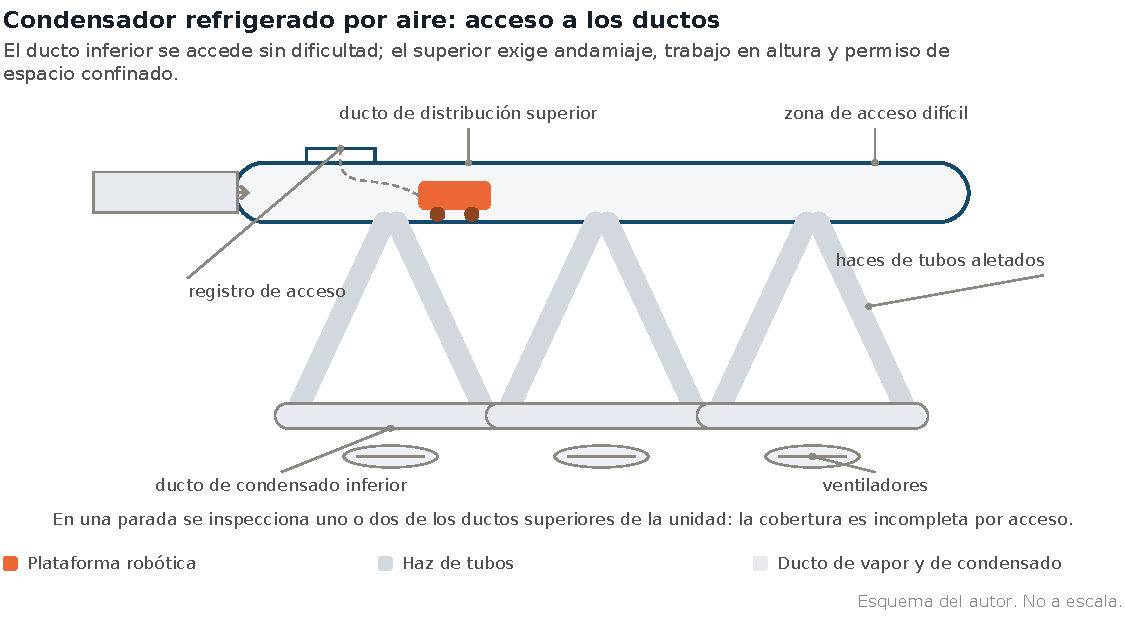
\includegraphics[width=0.98\linewidth]{assets/esq-acc.pdf}}
\caption*{\footnotesize\raggedright Figura 15 — Acceso a los ductos de un condensador refrigerado por aire. {\color{gray2}Esquema del autor.}}
\end{figure}

\subsubsection*{13.1 El problema, declarado por los propios operadores}
\addcontentsline{toc}{subsubsection}{13.1 El problema, declarado por los propios operadores}

\begin{notadato}{Dato verificado — guía de inspección interna de ACC \badge{sblue}{white}{B}}
La guía de inspección interna de la asociación de usuarios de condensadores refrigerados por aire establece que los ductos inferiores se acceden sin gran dificultad, pero que \textbf{es probablemente irreal esperar que se inspeccione más de uno o dos de los ductos superiores de una unidad durante una parada}, y recomienda que la planta elija un ducto superior específico.

Alcanzar ese ducto superior puede exigir andamiaje o escalera temporal y una trepada por barandas hasta el registro de acceso, con protección contra caídas. El ductwork se define como espacio confinado: exige aire respirable verificado, monitoreo durante la permanencia y plan de rescate, porque las riostras cruzadas pueden obstruir la extracción de una persona en una emergencia.

\end{notadato}
Esto invierte la formulación habitual del problema. \textbf{El dolor no es que la inspección sea cara: es que no se hace} sobre la mayor parte del activo, y la razón es el acceso.

El mecanismo de falla está documentado en la misma fuente: la corrosión del lado vapor transporta óxido de hierro al agua de alimentación de caldera, y las penetraciones pasantes en los tubos causan ingreso de aire con pérdida de rendimiento del condensador.


\subsubsection*{13.2 Escala del activo}
\addcontentsline{toc}{subsubsection}{13.2 Escala del activo}

Un condensador de este tipo puede tener del orden de 20.000 tubos y 40.000 soldaduras, y localizar una fuga puede equivaler a encontrar un orificio menor que una moneda en una superficie de tres o cuatro canchas de fútbol. \badge{lblue}{ink}{C} — cifra de prensa técnica especializada, no verificada de forma independiente.


\subsubsection*{13.3 Competencia identificada}
\addcontentsline{toc}{subsubsection}{13.3 Competencia identificada}

\begin{itemize}
\item \textbf{Conco Services} presta limpieza y detección de fugas con gas trazador. Resuelve la \textbf{localización de fugas desde el exterior}, no la evaluación interna del estado de corrosión. \badge{lblue}{ink}{C}
\item \textbf{EPRI} desarrolla una metodología con cámara acústica montada en dron para inspección de estos condensadores, sobre la base de resultados con cámara acústica de mano, y reporta ensayos con dron infrarrojo para analizar distribución de calor. \badge{sblue}{white}{B}
\item \textbf{No se identificó} ningún crawler ni robot de inspección interna de ductos de este activo después de las búsquedas registradas en la bitácora. Esto \textbf{no equivale} a afirmar que no exista.
\end{itemize}

\begin{notaclave}{Pregunta estratégica que decide el candidato}
¿Puede un robot inspeccionar los ductos superiores que hoy se dejan sin inspeccionar, con calidad suficiente para sustituir la entrada humana, y sin exigir el andamiaje que constituye la mayor parte del costo evitado?

Si la respuesta exige igualmente montar andamiaje para posicionar el robot, el caso se cae: el ahorro dejaría de ser el acceso y pasaría a ser sólo el tiempo de inspección.

\end{notaclave}

\subsubsection*{13.4 Por qué encaja con la plataforma existente}
\addcontentsline{toc}{subsubsection}{13.4 Por qué encaja con la plataforma existente}

Espacio confinado, tether, cámara e iluminación, mapeo y localización dentro de un ducto de sección constante, y generación automática de informe: la reutilización es alta y no exige un ensayo no destructivo nuevo, porque el hallazgo primario es visual y de estado de superficie.

\begin{detalle}{Agenda de verificación pendiente}
\begin{itemize}
\item Cuantificar cuántas unidades con condensador refrigerado por aire existen en el mercado objetivo y en la región, y su antigüedad.
\item Obtener el costo real de una parada con andamiaje para inspección de ducto superior, en al menos dos plantas.
\item Verificar si algún proveedor de limpieza o de detección de fugas ya ofrece inspección interna robotizada, aunque no la publique.
\item Screening de patentes sobre inspección interna de ductos de condensadores refrigerados por aire.
\item Determinar si el comprador es mantenimiento, química o ingeniería de activos, y quién firma la orden de compra.
\item Confirmar con la asociación de usuarios si la limitación de cobertura declarada en 2015 sigue vigente en 2026.
\end{itemize}

\end{detalle}

\subsection*{14. Mercados con madurez probablemente alta}
\addcontentsline{toc}{subsection}{14. Mercados con madurez probablemente alta}

No se descartan sin investigación, pero se exige evidencia de hueco antes de invertir en ellos.

\begin{tarjeta}{13.1 Robot nadador para transformadores}{\badge{lblue}{ink}{M4} \badge{lblue}{ink}{M5}}
Referencia de mercado: \textbf{ABB TXplore}, con inspección en menos de un día, eliminación de las tareas de drenaje y procesamiento de aceite y reducciones de costo declaradas de hasta aproximadamente 50 \% en comunicaciones del fabricante y casos publicados.

\textbf{Pregunta:} ¿hay algo que TXplore no haga y que tenga mercado independiente de ABB?

\end{tarjeta}
\begin{tarjeta}{13.2 Robots de patrulla de subestaciones}{\badge{lblue}{ink}{M4}}
EPRI trabaja con plataformas comerciales, incluido Spot de Boston Dynamics en determinados proyectos de subestaciones.

\textbf{Hipótesis:} el valor está más en la carga sensora y la analítica que en fabricar otro cuadrúpedo o vehículo terrestre no tripulado.

\end{tarjeta}
\begin{tarjeta}{13.3 Robots trepadores de línea de transmisión}{\badge{lblue}{ink}{M3}}
Debe investigarse el linaje completo: los desarrollos Ti de EPRI, LineScout y LineROVer de Hydro-Québec y el Expliner de HiBot, y determinar si los drones modernos hicieron económicamente obsoleto al crawler para inspección visual de rutina.

\end{tarjeta}
\begin{tarjeta}{13.4 Robots de inspección de tanques}{\badge{lblue}{ink}{M4} \badge{lblue}{ink}{M5}}
Square Robot, Newton Labs, Eddyfi y proveedores de vehículos submarinos operan hoy en tanques en servicio. Mercado probablemente maduro; se exige evidencia de hueco antes de considerarlo.

\end{tarjeta}
\begin{tarjeta}{13.5 Robótica de internos de reactor y tubos de generador de vapor}{\badge{lblue}{ink}{M5}}
Framatome, Westinghouse, la familia SUSI de AREVA y los desarrollos de KHNP/KEPRI cubren manipuladores de generador de vapor e internos de reactor. Mercado de altísimo valor, con proveedores establecidos y fuerte carga regulatoria: probablemente muy maduro.

\end{tarjeta}

\subsection*{15. Barrido de oportunidades fuera de la lista}
\addcontentsline{toc}{subsection}{15. Barrido de oportunidades fuera de la lista}

El estudio no se limita a los ocho candidatos: el barrido independiente es obligatorio y puede reordenar todo el ranking.


\subsubsection*{15.1 Resultado del barrido ejecutado}
\addcontentsline{toc}{subsubsection}{15.1 Resultado del barrido ejecutado}

El barrido se ejecutó por familias de activos y quedó registrado con sus consultas, fuentes y niveles de evidencia en la bitácora de investigación que acompaña a este informe. Resultado por familia:

\begingroup\footnotesize
\setlength{\tabcolsep}{4pt}
\setlength{\emergencystretch}{4em}
\hyphenpenalty=50 \exhyphenpenalty=50
\begin{longtable}{@{}>{\RaggedRight\arraybackslash}p{\dimexpr 0.3293\linewidth-2\tabcolsep\relax}>{\RaggedRight\arraybackslash}p{\dimexpr 0.2362\linewidth-2\tabcolsep\relax}>{\RaggedRight\arraybackslash}p{\dimexpr 0.4295\linewidth-2\tabcolsep\relax}@{}}
\toprule
\scriptsize\textbf{Familia de activos} & \scriptsize\textbf{Veredicto} & \scriptsize\textbf{Razón determinante} \\
\midrule
\endfirsthead
\toprule
\scriptsize\textbf{Familia de activos} & \scriptsize\textbf{Veredicto} & \scriptsize\textbf{Razón determinante} \\
\midrule
\endhead
\bottomrule
\endfoot
Condensadores refrigerados por aire & \textbf{Candidato nuevo (H)} & Cobertura de inspección incompleta declarada por los operadores; ningún robot identificado para el interior de los ductos \\
Paredes de agua de caldera e internos de hogar & No perseguir & Incumbente consolidado con producto, datos, canal y alianza con fabricante de calderas, más media docena de competidores \\
Eólica: palas, torres y monopilotes & No perseguir & Cuatro proveedores en el interior de la pala; el hueco restante está limitado por la atenuación del material \\
Presas, compuertas y válvulas & Refuerza al candidato F & Dolor documentado por el propietario del activo, pero el equipamiento base ya es comercial: el valor está en el paquete de servicio \\
Intercambiadores de calor, hornos y chimeneas & Descartado & Intercambiadores en mercado M5; hornos pertenecen a siderurgia, con otro canal y prior art de alta temperatura ya patentado \\
Aparamenta blindada y túneles de cables & Línea a investigar / no perseguir & Costo de intervención documentado en aparamenta pero búsqueda insuficiente; prior art abundante en túneles de cables \\
Solar y tareas nucleares del catálogo & Sin candidato, con dato clave & El valor en solar es analítica, no robótica; el catálogo nuclear aportó las horas-hombre por tarea de la sección 17 \\
\end{longtable}
\endgroup

\begin{notainferencia}{Cómo leer este resultado}
Seis de siete familias se cerraron por evidencia de ocupación del mercado o por una limitación física documentada. Ese es el rendimiento normal de un barrido honesto: la mayoría de las ideas atractivas ya fueron intentadas, y el valor del ejercicio está en descartarlas rápido y por escrito.

\end{notainferencia}

\subsubsection*{15.2 Barrido por programa sectorial}
\addcontentsline{toc}{subsubsection}{15.2 Barrido por programa sectorial}

Generación \textperiodcentered{} nuclear \textperiodcentered{} transmisión \textperiodcentered{} distribución \textperiodcentered{} hidroeléctrica \textperiodcentered{} combustibles fósiles y ciclo combinado \textperiodcentered{} eólica \textperiodcentered{} solar \textperiodcentered{} subestaciones \textperiodcentered{} transmisión subterránea \textperiodcentered{} modernización de plantas \textperiodcentered{} ensayos no destructivos \textperiodcentered{} transformación digital \textperiodcentered{} grupos de colaboración en robótica.


\subsubsection*{15.3 Tareas ya identificadas en la literatura sectorial}
\addcontentsline{toc}{subsubsection}{15.3 Tareas ya identificadas en la literatura sectorial}

EPRI 3002023899 identifica, entre otras, oportunidades de automatización en: tuberías enterradas de agua de servicio; soportes de componentes; estructuras de toma y descarga de agua de refrigeración; ducto de bus isofásico; mapeo tridimensional de radiación; detección de fugas en contención; espárragos y alojamientos de la tapa del reactor; tanques de almacenamiento de agua; contenedores de combustible en seco; rondas de operación; protección contra incendios; y tubos de generador de vapor.

\begin{notariesgo}{Esta lista no es una lista de productos}
Varias de esas tareas corresponden a mercados ya maduros. La lista sirve para orientar la búsqueda y para cruzarla con horas-hombre y brechas tecnológicas, no para elegir un producto.

\end{notariesgo}

\subsubsection*{15.4 Barrido por problema físico}
\addcontentsline{toc}{subsubsection}{15.4 Barrido por problema físico}

Espacio confinado \textperiodcentered{} inspección inaccesible \textperiodcentered{} inspección con rotor instalado \textperiodcentered{} sin desmontaje \textperiodcentered{} sin andamiaje \textperiodcentered{} sin excavación \textperiodcentered{} sin drenaje \textperiodcentered{} sin buceo \textperiodcentered{} sin desenergización \textperiodcentered{} en sitio \textperiodcentered{} inspección en línea \textperiodcentered{} inspección interna \textperiodcentered{} ensayos no destructivos robotizados y remotos \textperiodcentered{} inspección autónoma \textperiodcentered{} inspección combinada con reparación \textperiodcentered{} inspección combinada con limpieza \textperiodcentered{} recuperación de material extraño.


\subsubsection*{15.5 Activos adicionales a evaluar}
\addcontentsline{toc}{subsubsection}{15.5 Activos adicionales a evaluar}

Condensadores refrigerados por aire \textperiodcentered{} condensadores \textperiodcentered{} torres de refrigeración \textperiodcentered{} paredes de agua de caldera \textperiodcentered{} headers de caldera \textperiodcentered{} internos de hogar \textperiodcentered{} zonas de escape y combustión de turbina de gas \textperiodcentered{} internos de turbina de vapor \textperiodcentered{} palas y torres de aerogeneradores \textperiodcentered{} monopilotes marinos \textperiodcentered{} presas \textperiodcentered{} vertederos \textperiodcentered{} compuertas de toma \textperiodcentered{} válvulas de gran tamaño \textperiodcentered{} intercambiadores de calor \textperiodcentered{} chimeneas \textperiodcentered{} hornos industriales \textperiodcentered{} recipientes y tuberías petroquímicas \textperiodcentered{} activos mineros cuando la tecnología sea transferible.

\clearpage

\section*{Parte III — Método de evaluación y economía}
\addcontentsline{toc}{section}{Parte III — Método de evaluación y economía}


\subsection*{16. Ficha estándar por candidato}
\addcontentsline{toc}{subsection}{16. Ficha estándar por candidato}

Todos los candidatos se documentan con la misma ficha de 23 campos. La uniformidad es lo que permite comparar; una ficha incompleta se marca como incompleta y no se completa con supuestos.

\begin{tarjeta}{1 \textperiodcentered{} Activo y problema}{}
Qué se inspecciona, cuál es el mecanismo de falla y por qué importa para la operación.

\end{tarjeta}
\begin{tarjeta}{2 \textperiodcentered{} Cómo se inspecciona hoy}{}
Rotor extraído, desmontaje, andamiaje, buceo, entrada de personal; frecuencia, duración, personal, salida de servicio y riesgos.

\end{tarjeta}
\begin{tarjeta}{3 \textperiodcentered{} Dolor económico verificable}{}
Costo directo, costo de parada, costo de acceso, horas-hombre, pérdida por falla y ejemplos reales. Separando dato publicado de estimación.

\end{tarjeta}
\begin{tarjeta}{4 \textperiodcentered{} Propuesta de robot}{}
Locomoción, dimensiones aproximadas, sensores, ensayo no destructivo, tether o inalámbrico, autonomía, mapeo y localización, manipulación y recuperación. A nivel de requisitos, no de diseño.

\end{tarjeta}
\begin{tarjeta}{5 \textperiodcentered{} Valor creado}{}
Qué operación evita, cuánto tiempo reduce, cuánta cobertura agrega, cuánta confiabilidad mejora y cuánto riesgo disminuye.

\end{tarjeta}
\begin{tarjeta}{6 \textperiodcentered{} Robots y productos existentes}{}
Registro obligatorio en tabla, incluyendo productos vivos, sistemas sólo de servicio, prototipos, discontinuados y patentes.

\end{tarjeta}
\begin{tarjeta}{7 \textperiodcentered{} Cómo lo resolvieron los existentes}{}
Adhesión, ruedas, orugas o magnetismo, arquitectura serpiente o continua, tether, energía, acoplamiento del sensor, contacto del ensayo, superación de obstáculos, alineación, recuperación y material extraño.

\end{tarjeta}
\begin{tarjeta}{8 \textperiodcentered{} Qué no resuelven}{}
Identificación del hueco real. Es el campo que decide si hay producto.

\end{tarjeta}
\begin{tarjeta}{9 \textperiodcentered{} Mercado y madurez}{}
Posición en la escala M0–M5, sin confundir nivel tecnológico con madurez comercial.

\end{tarjeta}
\begin{tarjeta}{10 \textperiodcentered{} Barreras técnicas}{}
Geometría, temperatura, radiación, interferencia electromagnética, fluidos, suciedad, corrosión, tether, adhesión, batería, sensado y calibración del ensayo.

\end{tarjeta}
\begin{tarjeta}{11 \textperiodcentered{} Riesgo de atascamiento y recuperación}{}
Filosofía de falla segura y procedimiento de recuperación como parte del producto.

\end{tarjeta}
\begin{tarjeta}{12 \textperiodcentered{} Regulación y calificación}{}
Ámbito nuclear, calificación de ensayos no destructivos, alta tensión, espacio confinado, frontera de presión y códigos aplicables.

\end{tarjeta}
\begin{tarjeta}{13 \textperiodcentered{} Patentes y propiedad intelectual}{}
Familias principales, titulares, estado legal, riesgo de bloqueo y áreas posiblemente libres.

\end{tarjeta}
\begin{tarjeta}{14 \textperiodcentered{} Desarrollo estimado}{}
Separado en plataforma, carga sensora, ensayo no destructivo, software, calificación y validación de campo. Con rango y justificación.

\end{tarjeta}
\begin{tarjeta}{15 \textperiodcentered{} Modelo de negocio}{}
Venta, alquiler, servicio, precio por inspección, contrato anual o suscripción de datos y analítica.

\end{tarjeta}
\begin{tarjeta}{16 \textperiodcentered{} Cliente y comprador}{}
Utility, fabricante, contratista de parada, empresa de ensayos, aseguradora o propietario del activo. Debe identificarse quién firma la orden de compra.

\end{tarjeta}
\begin{tarjeta}{17 \textperiodcentered{} Frecuencia de compra}{}
Fundamentada con evidencia, no supuesta.

\end{tarjeta}
\begin{tarjeta}{18 \textperiodcentered{} Tamaño de mercado}{}
Sólo si hay datos suficientes. Separado en global, Estados Unidos, Latinoamérica y Argentina.

\end{tarjeta}
\begin{tarjeta}{19 \textperiodcentered{} Precio y \hyperlink{g-ticket}{ticket}\textsuperscript{\textsc{g}}}{}
Precios publicados, licitaciones, contratos, cotizaciones o comparables. No se inventa.

\end{tarjeta}
\begin{tarjeta}{20 \textperiodcentered{} Reutilización de la plataforma existente}{}
Puntuación por subsistema: locomoción, cómputo, cámaras, iluminación, tether, lógica programable, encoders, software, mapeo, generación de informes y arquitectura de seguridad.

\end{tarjeta}
\begin{tarjeta}{21 \textperiodcentered{} Defensa posible}{}
Mecánica, ensayo no destructivo, conjunto de datos, calibración, software, calificación, flujo de trabajo de servicio y patentes.

\end{tarjeta}
\begin{tarjeta}{22 \textperiodcentered{} \hyperlink{g-go-nogo}{Decisión de avance}\textsuperscript{\textsc{g}}}{}
Avanzar o no avanzar, con conclusión breve y sin ambigüedad.

\end{tarjeta}
\begin{tarjeta}{23 \textperiodcentered{} Confianza}{}
Alta, media o baja, explicando qué dato falta para elevarla.

\end{tarjeta}

\subsubsection*{16.1 Registro obligatorio de productos existentes}
\addcontentsline{toc}{subsubsection}{16.1 Registro obligatorio de productos existentes}

\begin{landscape}
\begingroup\footnotesize
\setlength{\tabcolsep}{2pt}
\setlength{\emergencystretch}{4em}
\hyphenpenalty=50 \exhyphenpenalty=50
\begin{longtable}{@{}>{\RaggedRight\arraybackslash}p{\dimexpr 0.0942\linewidth-2\tabcolsep\relax}>{\RaggedRight\arraybackslash}p{\dimexpr 0.1177\linewidth-2\tabcolsep\relax}>{\RaggedRight\arraybackslash}p{\dimexpr 0.0453\linewidth-2\tabcolsep\relax}>{\RaggedRight\arraybackslash}p{\dimexpr 0.0706\linewidth-2\tabcolsep\relax}>{\RaggedRight\arraybackslash}p{\dimexpr 0.1177\linewidth-2\tabcolsep\relax}>{\RaggedRight\arraybackslash}p{\dimexpr 0.1161\linewidth-2\tabcolsep\relax}>{\RaggedRight\arraybackslash}p{\dimexpr 0.1295\linewidth-2\tabcolsep\relax}>{\RaggedRight\arraybackslash}p{\dimexpr 0.1295\linewidth-2\tabcolsep\relax}>{\RaggedRight\arraybackslash}p{\dimexpr 0.1039\linewidth-2\tabcolsep\relax}>{\RaggedRight\arraybackslash}p{\dimexpr 0.0706\linewidth-2\tabcolsep\relax}@{}}
\toprule
\scriptsize\textbf{Producto} & \scriptsize\textbf{Fabricante} & \scriptsize\textbf{Año} & \scriptsize\textbf{Estado 2026} & \scriptsize\textbf{Locomoción} & \scriptsize\textbf{Carga sensora \slash  NDE} & \scriptsize\textbf{Dimensiones} & \scriptsize\textbf{Despliegues} & \scriptsize\textbf{Precio o servicio} & \scriptsize\textbf{Fuente} \\
\midrule
\endfirsthead
\toprule
\scriptsize\textbf{Producto} & \scriptsize\textbf{Fabricante} & \scriptsize\textbf{Año} & \scriptsize\textbf{Estado 2026} & \scriptsize\textbf{Locomoción} & \scriptsize\textbf{Carga sensora \slash  NDE} & \scriptsize\textbf{Dimensiones} & \scriptsize\textbf{Despliegues} & \scriptsize\textbf{Precio o servicio} & \scriptsize\textbf{Fuente} \\
\midrule
\endhead
\bottomrule
\endfoot
\multicolumn{10}{@{}l@{}}{\itshape Plantilla de registro: se completa durante la investigación.} \\
\end{longtable}
\endgroup
\end{landscape}


\subsection*{17. Dimensionamiento de mercado}
\addcontentsline{toc}{subsection}{17. Dimensionamiento de mercado}

No se usan como base informes genéricos del tipo «mercado de robots de inspección». El cálculo se construye \textbf{\hyperlink{g-bottom-up}{de abajo hacia arriba}\textsuperscript{\textsc{g}}}, y su resultado es el mercado total direccionable de servicios (\hyperlink{g-tam}{TAM}\textsuperscript{\textsc{g}}):

\texttt{Activos direccionables $\times$ inspecciones por año $\times$ ticket de servicio = mercado de servicios}

Se publican tres escenarios —bajo, base y alto— con la fuente de cada entrada. \textbf{Si falta información crítica, no se fabrica el número.}


\subsubsection*{17.1 Anclaje verificado: horas-hombre por tarea}
\addcontentsline{toc}{subsubsection}{17.1 Anclaje verificado: horas-hombre por tarea}

EPRI publica, a partir del análisis de su base de órdenes de trabajo, el consumo de horas-hombre por caso de uso. Es el punto de partida para el cálculo de abajo hacia arriba del costo evitado, y evita construir el dimensionamiento sobre supuestos propios.

\begingroup\footnotesize
\setlength{\tabcolsep}{4pt}
\setlength{\emergencystretch}{4em}
\hyphenpenalty=50 \exhyphenpenalty=50
\begin{longtable}{@{}>{\RaggedRight\arraybackslash}p{\dimexpr 0.3163\linewidth-2\tabcolsep\relax}>{\RaggedRight\arraybackslash}p{\dimexpr 0.3451\linewidth-2\tabcolsep\relax}>{\RaggedRight\arraybackslash}p{\dimexpr 0.3336\linewidth-2\tabcolsep\relax}@{}}
\toprule
\scriptsize\textbf{Caso de uso} & \scriptsize\textbf{Frecuencia declarada} & \scriptsize\textbf{Horas-hombre por unidad y por año} \\
\midrule
\endfirsthead
\toprule
\scriptsize\textbf{Caso de uso} & \scriptsize\textbf{Frecuencia declarada} & \scriptsize\textbf{Horas-hombre por unidad y por año} \\
\midrule
\endhead
\bottomrule
\endfoot
Tuberías de agua de servicio, enterradas y sobre nivel & Inspección dirigida cada 10 años; cada 3 a 5 años en la década previa al fin de vida de diseño & 5.000 a 10.000 \\
Estructuras de toma y descarga de agua de refrigeración & Entre anual y cada 5 años, según condición observada & 50 a 1.500, con el rango gobernado por la calidad del agua \\
Rondas de operación & Diarias & $\approx$ 1.400, unas 4 horas por día \\
Vigilancia contra incendios & Variable, de semanal a mayor & 500 a 1.500 \\
Mapa tridimensional de radiación & Línea de base cada 10 años & 250 a 750 en trabajo emergente \\
Tanques de almacenamiento de agua & Inspección completa en cada período de 10 años & 50 a 500, tanques de condensado \\
Espárragos y alojamientos de la tapa del reactor & Aproximadamente cada parada & 150 o más por parada \\
Detección de fugas en contención & Emergente, creciente con la edad de la planta & $\approx$ 50 \\
Tubos de generador de vapor & Cada parada o cada dos paradas & $\approx$ 50 con la tecnología existente \\
\end{longtable}
\endgroup

Fuente: EPRI, \emph{Robotic Process Automation for Nuclear Power Plants: Evaluation of Near-Term Opportunities}, 3002023899, junio 2022, tablas 1 a 12. \badge{navy}{white}{A}

\begin{notainferencia}{Qué dice esta tabla sobre dónde está el negocio}
Las mayores bolsas de horas no corresponden a las tareas más difíciles: tuberías de agua de servicio, rondas de operación y vigilancia contra incendios concentran mucho más tiempo que las inspecciones especializadas. Pero son tareas de alta frecuencia y baja complejidad, que compiten contra plataformas de propósito general ya comerciales.

El negocio del tipo de robot que este estudio evalúa no está en las horas totales sino en el \textbf{costo evitado por intervención}: parada, andamiaje, excavación, buceo o izaje pesado. La tabla sirve para dimensionar, no para elegir.

\end{notainferencia}

\subsubsection*{17.2 Fuentes preferidas por región}
\addcontentsline{toc}{subsubsection}{17.2 Fuentes preferidas por región}

\begin{tarjeta}{Estados Unidos}{}
EIA, NRC, DOE, FERC y NERC; informes públicos de utilities; y EPRI.

\end{tarjeta}
\begin{tarjeta}{Nuclear global}{}
Base de datos PRIS del OIEA como fuente primaria; la World Nuclear Association sólo como fuente secundaria.

\end{tarjeta}
\begin{tarjeta}{Argentina}{}
CAMMESA, Secretaría de Energía, ENRE, Nucleoeléctrica Argentina, Transener, empresas generadoras y operadores de ciclo combinado e hidroeléctricos.

\end{tarjeta}
\begin{tarjeta}{Latinoamérica}{}
Ministerios, operadores de sistema y utilities; OLADE y CIER; siempre sobre bases públicas verificables.

\end{tarjeta}

\subsection*{18. Economía del cliente}
\addcontentsline{toc}{subsection}{18. Economía del cliente}

El análisis mira la decisión desde el lado del cliente, no desde el costo del producto.

\begin{figure}[htbp]\centering
\fbox{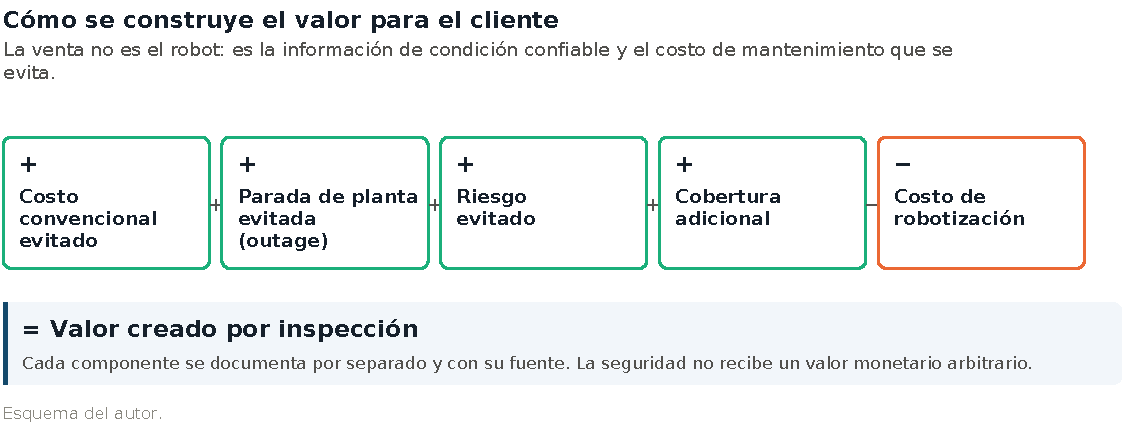
\includegraphics[width=0.98\linewidth]{assets/fig-valor.pdf}}
\caption*{\footnotesize\raggedright Figura 16 — Componentes del valor creado por una inspección robotizada. {\color{gray2}Elaboración propia.}}
\end{figure}
Cada componente se documenta por separado y con su fuente. \textbf{No se asigna valor monetario arbitrario a la seguridad}: se declara como beneficio no monetizado cuando no hay base para cuantificarlo.

Se buscan ejemplos reales y verificables de: días de parada, andamiaje, excavación, vaciado de conducto, drenaje de tanque, extracción de rotor, entrada de personal a espacio confinado, operación de buceo y maniobras de izaje pesado.


\subsection*{19. Rankings y análisis de sensibilidad}
\addcontentsline{toc}{subsection}{19. Rankings y análisis de sensibilidad}

Se construyen dos rankings con criterios distintos, porque responden a preguntas distintas: cuál es el mejor próximo producto (\hyperlink{g-fast-follow}{seguidor rápido}\textsuperscript{\textsc{g}}) y cuál es la posición más defendible a largo plazo (\hyperlink{g-moat}{moat}\textsuperscript{\textsc{g}}, con su \hyperlink{g-upside}{potencial de crecimiento}\textsuperscript{\textsc{g}}).

\begin{figure}[htbp]\centering
\fbox{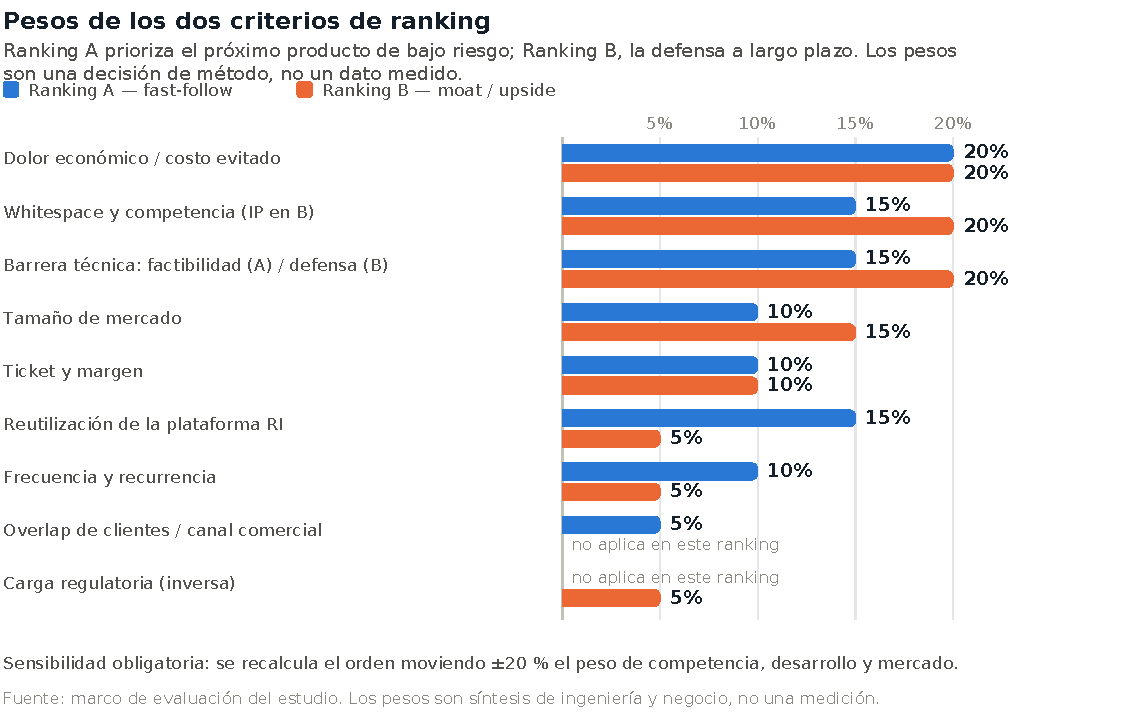
\includegraphics[width=0.98\linewidth]{assets/fig-pesos.pdf}}
\caption*{\footnotesize\raggedright Figura 17 — Pesos comparados de los criterios en ambos rankings. {\color{gray2}Elaboración propia; los pesos son una decisión de método.}}
\end{figure}
\begin{notainferencia}{Los puntajes no son mediciones}
Los puntajes son una \textbf{síntesis de ingeniería y de negocio}, y así deben etiquetarse en el informe. Los pesos pueden modificarse si se justifica el cambio, pero entonces debe recalcularse el orden completo.

\end{notainferencia}

\subsubsection*{19.1 Sensibilidad obligatoria}
\addcontentsline{toc}{subsubsection}{19.1 Sensibilidad obligatoria}

En el \hyperlink{g-sensibilidad}{análisis de sensibilidad}\textsuperscript{\textsc{g}} se recalcula el ranking moviendo $\pm$20 \% el peso de competencia, de esfuerzo de desarrollo y de tamaño de mercado. Si el ganador cambia con esas variaciones, la recomendación debe declararse \textbf{inestable} y la decisión debe esperar a la evidencia que estabilice el criterio dominante.


\subsection*{20. Prior art, patentes y competidores}
\addcontentsline{toc}{subsection}{20. Prior art, patentes y competidores}


\subsubsection*{20.1 Screening preliminar de propiedad intelectual}
\addcontentsline{toc}{subsubsection}{20.1 Screening preliminar de propiedad intelectual}

Para los cinco candidatos mejor posicionados se realiza búsqueda formal en Google Patents, Espacenet, WIPO Patentscope y USPTO, combinando el activo con: inspección robótica, crawler, inspección remota, ensayo no destructivo, trepado de paredes, robot serpiente, vehículo de inspección y manipulador.

\begingroup\footnotesize
\setlength{\tabcolsep}{3pt}
\setlength{\emergencystretch}{4em}
\hyphenpenalty=50 \exhyphenpenalty=50
\begin{longtable}{@{}>{\RaggedRight\arraybackslash}p{\dimexpr 0.1361\linewidth-2\tabcolsep\relax}>{\RaggedRight\arraybackslash}p{\dimexpr 0.1750\linewidth-2\tabcolsep\relax}>{\RaggedRight\arraybackslash}p{\dimexpr 0.1361\linewidth-2\tabcolsep\relax}>{\RaggedRight\arraybackslash}p{\dimexpr 0.1944\linewidth-2\tabcolsep\relax}>{\RaggedRight\arraybackslash}p{\dimexpr 0.1211\linewidth-2\tabcolsep\relax}>{\RaggedRight\arraybackslash}p{\dimexpr 0.2322\linewidth-2\tabcolsep\relax}@{}}
\toprule
\scriptsize\textbf{Familia} & \scriptsize\textbf{Prioridad} & \scriptsize\textbf{Titular} & \scriptsize\textbf{Qué reivindica} & \scriptsize\textbf{Estado legal} & \scriptsize\textbf{Riesgo para el proyecto} \\
\midrule
\endfirsthead
\toprule
\scriptsize\textbf{Familia} & \scriptsize\textbf{Prioridad} & \scriptsize\textbf{Titular} & \scriptsize\textbf{Qué reivindica} & \scriptsize\textbf{Estado legal} & \scriptsize\textbf{Riesgo para el proyecto} \\
\midrule
\endhead
\bottomrule
\endfoot
\multicolumn{6}{@{}l@{}}{\itshape Plantilla de registro: se completa durante la investigación.} \\
\end{longtable}
\endgroup

\begin{notariesgo}{Alcance del análisis}
Esto \textbf{no} constituye una opinión legal de libertad de operación. Es un screening preliminar orientado a detectar bloqueos evidentes y áreas potencialmente libres.

\end{notariesgo}

\subsubsection*{20.2 Mapa de actores por oportunidad}
\addcontentsline{toc}{subsubsection}{20.2 Mapa de actores por oportunidad}

Para cada oportunidad se identifican por separado seis papeles, porque rara vez los cumple la misma empresa:

\begin{enumerate}
\item \textbf{Fabricante del robot}: quién construye el hardware.
\item \textbf{Proveedor del ensayo no destructivo}: quién fabrica o posee el sensor.
\item \textbf{Empresa de servicio}: quién vende efectivamente la inspección.
\item \textbf{Integrador}: quién combina plataforma y sensor.
\item \textbf{Tecnología desarrollada por la utility}: si el cliente resolvió el problema internamente.
\item \textbf{Derivación universitaria}: si existe una empresa surgida de un grupo de investigación.
\end{enumerate}

Se registra además el historial de adquisiciones —un producto puede haber cambiado de dueño o de nombre— y el estado a 2026: activo, discontinuado, adquirido, sin comercialización o indeterminado. Para productos desaparecidos se recurre al Internet Archive y a folletos archivados; las redes profesionales se usan sólo como pista inicial, nunca como evidencia.


\subsubsection*{20.3 Licitaciones y contratos como fuente de verdad comercial}
\addcontentsline{toc}{subsubsection}{20.3 Licitaciones y contratos como fuente de verdad comercial}

Un contrato adjudicado dice más sobre el mercado que cualquier informe de tamaño de mercado. Se buscan \hyperlink{g-licitacion}{licitaciones, pedidos de cotización}\textsuperscript{\textsc{g}} y adjudicaciones reales por servicio de inspección, inspección robótica, bus isofásico, inspección de HRSG, inspección de vaults, tuberías enterradas, conductos forzados, contenedores en seco, crawlers e inspección visual remota, en portales oficiales de compras de utilities, estatales, federales, municipales y nucleares cuando sean públicos.

De cada uno se extrae: alcance, frecuencia, requisitos, duración, monto adjudicado si aparece y proveedor ganador.


\subsection*{21. Argentina y Latinoamérica}
\addcontentsline{toc}{subsection}{21. Argentina y Latinoamérica}

Para los tres candidatos mejor posicionados se desarrolla un capítulo específico que responde:

\begin{enumerate}
\item ¿Cuántos activos de ese tipo existen en Argentina?
\item ¿Quiénes los operan?
\item ¿Quién realiza hoy la inspección?
\item ¿Se contrata al fabricante internacional o a un servicio local?
\item ¿Podría prestarse el servicio regional desde Argentina?
\item ¿Qué requisitos de importación y calibración implica?
\item ¿Existen integradores o socios locales de ensayos no destructivos?
\item ¿Hay centrales con equipamiento de los grandes fabricantes donde el canal comercial sea similar al del producto de referencia?
\item ¿Qué mercados vecinos son naturales: Brasil, Chile, Uruguay, Paraguay, Perú, Colombia o México?
\end{enumerate}

Las cantidades se toman de fuentes oficiales del sector y de los operadores. \textbf{No se estiman cantidades de activos sin fuente.}


\subsection*{22. Costos de desarrollo}
\addcontentsline{toc}{subsection}{22. Costos de desarrollo}

Para cada candidato de la lista corta se estima por separado: diseño mecánico, prototipo, electrónica, sensores y ensayos no destructivos, tether y alimentación, software y control, navegación autónoma, gestión de datos e informes, banco de pruebas, maqueta de ensayo, calificación de campo, certificación y utillaje de fabricación.

Se prefieren \textbf{rangos amplios antes que falsa precisión}, y se distinguen cuatro magnitudes que suelen confundirse:

\begin{itemize}
\item costo de construir un prototipo;
\item \hyperlink{g-nre}{ingeniería no recurrente}\textsuperscript{\textsc{g}} para industrializar;
\item costo unitario aproximado en producción;
\item costo del kit de servicio de campo.
\end{itemize}

Se buscan precios reales de los componentes críticos siempre que sea posible.

\clearpage

\section*{Parte IV — Entregables, validación y cierre}
\addcontentsline{toc}{section}{Parte IV — Entregables, validación y cierre}


\subsection*{23. Estructura y requisitos del informe final}
\addcontentsline{toc}{subsection}{23. Estructura y requisitos del informe final}


\subsubsection*{23.1 Estructura}
\addcontentsline{toc}{subsubsection}{23.1 Estructura}

El informe final se organiza en: portada; resumen ejecutivo de tres páginas como máximo; objetivo y alcance; metodología y evidencia; qué hace atractivo un negocio de robótica de inspección; mapa completo de oportunidades; fichas por candidato; panorama competitivo transversal; panorama de patentes; mercado global, de Estados Unidos, de Latinoamérica y de Argentina; economía del cliente; matriz de comparación; rankings con sensibilidad; conceptos de producto para los tres primeros; lista de oportunidades a no perseguir por ahora; incógnitas y \hyperlink{g-due-diligence}{debida diligencia}\textsuperscript{\textsc{g}} pendiente; conclusiones; y anexos de registro de búsquedas, competidores, patentes y fuentes.


\subsubsection*{23.2 Requisitos de presentación}
\addcontentsline{toc}{subsubsection}{23.2 Requisitos de presentación}

\begin{tarjeta}{Estilo}{}
Limpio, técnico y ejecutivo. Legible y adaptable a pantalla e impresión. Tablas largas con encabezado fijo, índice navegable y llamados diferenciados para hallazgo, riesgo, inferencia y dato verificado. Sin saturación de color.

\end{tarjeta}
\begin{tarjeta}{Componentes}{}
Tarjetas de resultado ejecutivo, matriz de comparación, notas de fuente desplegables, distintivos de nivel de evidencia A–D, de madurez M0–M5 y de confianza.

\end{tarjeta}
\begin{tarjeta}{Gráficos requeridos}{}
Valor frente a madurez de mercado; reutilización de plataforma frente a dificultad de desarrollo; comparación de puntajes; línea temporal de prior art de los tres primeros; economía del cliente convencional frente a robotizada cuando existan cifras reales; y panorama de proveedores por oportunidad.

\end{tarjeta}
\begin{tarjeta}{Qué evitar}{}
Lenguaje de marketing, afirmaciones sin sustento, imágenes decorativas, gráficos tridimensionales, tablas ilegibles y relleno sin contenido.

\end{tarjeta}
Toda gráfica debe indicar su fuente, diferenciar dato de puntaje y no inventar precisión numérica.


\subsubsection*{23.3 Imágenes}
\addcontentsline{toc}{subsubsection}{23.3 Imágenes}

Se usan imágenes cuando ayudan a entender geometría del activo, robot existente, mecanismo de acceso, herramienta de ensayo o arquitectura propuesta, con este orden de preferencia: instituto de investigación sectorial, fabricante, caso de utility, literatura técnica y patente. Cada imagen lleva epígrafe, sistema y fabricante, fuente, dirección y fecha de consulta.

Si la licencia no permite incorporación confiable, se enlaza la fuente o se elabora un esquema original claramente identificado como tal, como los de este documento. Los archivos gráficos se guardan localmente para que el informe sea autocontenido.


\subsubsection*{23.4 Referencias}
\addcontentsline{toc}{subsubsection}{23.4 Referencias}

Las referencias se colocan junto a la afirmación que sostienen, no en una bibliografía desconectada. Ejemplo del formato esperado:

\begin{quote}\itshape EPRI reporta que una utility pagó aproximadamente USD 100.000 por una implementación de inspección robótica de bus isofásico y que la ejecución tomó menos de un día [EPRI-MTA-029].\end{quote}
Cada referencia registra organización o autor, título, fecha, identificador de producto, DOI o número de patente, dirección, fecha de acceso y nivel de evidencia.


\subsubsection*{23.5 Archivos que componen la entrega}
\addcontentsline{toc}{subsubsection}{23.5 Archivos que componen la entrega}

\begin{itemize}
\item informe completo en formato navegable;
\item registro de fuentes con nota de qué sostiene cada una;
\item tabla de evidencia con candidato, afirmación, valor, unidad, identificador de fuente, tipo, nivel, dirección, fecha de acceso, confianza y notas;
\item tabla de competidores con producto, empresa, aplicación, estado, país, tecnología, dimensiones, carga sensora, despliegues, precio y fuente;
\item tabla de patentes;
\item carpeta de imágenes y gráficos generados;
\item registro de investigación con consultas realizadas, bases consultadas, pistas descartadas y fuentes que no pudieron obtenerse.
\end{itemize}


\subsection*{24. Preguntas que el informe debe responder}
\addcontentsline{toc}{subsection}{24. Preguntas que el informe debe responder}

\begin{tarjeta}{Decisión}{}
\begin{enumerate}
\item Si hubiera que invertir hoy en un solo robot después del producto de referencia, ¿cuál sería?
\item ¿Por qué pagaría un cliente por él?
\item ¿Qué costo concreto se le evita?
\item ¿Qué ticket de servicio puede sostener?
\item ¿Cuántas oportunidades de servicio existen por año?
\end{enumerate}

\end{tarjeta}
\begin{tarjeta}{Competencia}{}
\begin{enumerate}[start=6]
\item ¿Quién hace esto hoy?
\item ¿Por qué el producto propuesto sería mejor o diferente?
\item ¿Qué tan difícil es copiarlo?
\item ¿Qué propiedad intelectual puede bloquearlo?
\end{enumerate}

\end{tarjeta}
\begin{tarjeta}{Ejecución}{}
\begin{enumerate}[start=10]
\item ¿Qué parte de la plataforma actual se reutiliza?
\item ¿Cuánto desarrollo falta?
\item ¿Cuál es el primer \hyperlink{g-mvp}{producto mínimo viable}\textsuperscript{\textsc{g}} que un cliente pagaría por probar?
\item ¿Qué validación técnica sería suficiente?
\item ¿Cuál es el principal mecanismo de fracaso?
\end{enumerate}

\end{tarjeta}
\begin{tarjeta}{Alcance}{}
\begin{enumerate}[start=15]
\item ¿Qué robot no debería desarrollarse aunque parezca atractivo?
\item ¿Qué oportunidad nueva apareció durante la investigación?
\item ¿Qué información no existe públicamente y requiere entrevistas?
\item ¿A qué diez personas u organizaciones debería contactarse primero?
\end{enumerate}

\end{tarjeta}

\subsection*{25. Programa de entrevistas}
\addcontentsline{toc}{subsection}{25. Programa de entrevistas}

Para los tres candidatos mejor posicionados se define una lista concreta de entrevistas de \hyperlink{g-customer-discovery}{descubrimiento de clientes}\textsuperscript{\textsc{g}}. Los perfiles a cubrir son: responsable de mantenimiento de generadores; responsable de paradas; responsable de ensayos no destructivos; jefe de planta; ingeniero de cables de transmisión; especialista en calderas de recuperación; responsable de servicio del fabricante de equipos; líder técnico del instituto de investigación sectorial; proveedor de servicios de ensayos no destructivos; e ingeniero de riesgo o de seguros cuando aplique.

Se preparan entre 8 y 12 preguntas por segmento, orientadas a: costo actual, frecuencia, dolor operativo, fallas sufridas, disposición a pagar, requisitos de aceptación, recuperación de herramienta y material extraño, proceso de compra e incumbente.


\subsection*{26. Criterio de finalización}
\addcontentsline{toc}{subsection}{26. Criterio de finalización}

El informe no se cierra porque «haya suficiente información». Se cierra cuando esta lista está completa:

\begin{itemize}[label=$\square$,leftmargin=1.6em]
\item Se recorrió el índice completo de productos de robótica y tecnologías móviles del instituto sectorial.
\item Se recorrió el catálogo de modernización de plantas buscando robótica e inspección.
\item Se buscó cada activo combinado con robótica.
\item Se buscó cada activo \textbf{sin} la palabra robot, para encontrar métodos competidores.
\item Se investigaron al menos los ocho candidatos principales.
\item Se buscaron candidatos nuevos fuera de la lista inicial.
\item Se hizo búsqueda profunda de competidores para los cinco primeros.
\item Se hizo screening de patentes para los cinco primeros.
\item Se buscaron licitaciones y contratos para los tres primeros.
\item Se verificó el estado 2026 de cada competidor principal.
\item Se buscó precio o ticket cuando existe.
\item Cada número relevante tiene referencia inmediata.
\item Cada afirmación de fabricante está etiquetada como tal.
\item Cada inferencia está etiquetada como tal.
\item Se documentó la evidencia negativa encontrada.
\item Se hizo dimensionamiento de mercado de abajo hacia arriba, o se explicó por qué no es defendible.
\item Se desarrolló el capítulo de Argentina y Latinoamérica para los tres primeros.
\item Se hizo el análisis de sensibilidad del ranking.
\item Se definieron los tres candidatos principales.
\item Se definió la lista de oportunidades a no perseguir por ahora.
\item Se listaron las incógnitas pendientes.
\item Se listaron las entrevistas y contactos prioritarios.
\item Se verificó que el informe sea autocontenido y abra correctamente.
\end{itemize}


\subsection*{27. Conclusión operativa}
\addcontentsline{toc}{subsection}{27. Conclusión operativa}

\begin{notaclave}{Principio rector}
La prioridad no es defender una solución: es no enamorarse de ninguna. Si la evidencia muestra que el bus isofásico está saturado, que el incumbente de HRSG cerró el hueco, que la robótica de vaults no tiene economía, que existe un producto desconocido que invalida la propuesta o que otra aplicación ofrece un negocio mucho mejor, \textbf{el ranking cambia}.

\end{notaclave}
El resultado debe permitir tomar una decisión de inversión con tres cosas claramente separadas: lo que sabemos, lo que inferimos y lo que todavía debemos validar. Y la conclusión debe responder sin ambigüedad cuál debería ser el próximo robot a desarrollar, y por qué.

\clearpage

\section*{Anexos}
\addcontentsline{toc}{section}{Anexos}


\subsection*{Anexo A — Paquete de fuentes verificado}
\addcontentsline{toc}{subsection}{Anexo A — Paquete de fuentes verificado}

Fuentes iniciales verificadas a la fecha de corte. No reemplazan la investigación: son el punto de partida.

\begingroup\footnotesize
\setlength{\tabcolsep}{3pt}
\setlength{\emergencystretch}{4em}
\hyphenpenalty=50 \exhyphenpenalty=50
\begin{longtable}{@{}>{\RaggedRight\arraybackslash}p{\dimexpr 0.0490\linewidth-2\tabcolsep\relax}>{\RaggedRight\arraybackslash}p{\dimexpr 0.2941\linewidth-2\tabcolsep\relax}>{\RaggedRight\arraybackslash}p{\dimexpr 0.2941\linewidth-2\tabcolsep\relax}>{\RaggedRight\arraybackslash}p{\dimexpr 0.0637\linewidth-2\tabcolsep\relax}>{\RaggedRight\arraybackslash}p{\dimexpr 0.2941\linewidth-2\tabcolsep\relax}@{}}
\toprule
\scriptsize\textbf{\#} & \scriptsize\textbf{Fuente} & \scriptsize\textbf{Referencia y dirección} & \scriptsize\textbf{Nivel} & \scriptsize\textbf{Qué sostiene} \\
\midrule
\endfirsthead
\toprule
\scriptsize\textbf{\#} & \scriptsize\textbf{Fuente} & \scriptsize\textbf{Referencia y dirección} & \scriptsize\textbf{Nivel} & \scriptsize\textbf{Qué sostiene} \\
\midrule
\endhead
\bottomrule
\endfoot
1 & EPRI — \emph{Robotic Process Automation for Nuclear Power Plants: Evaluation of Near-Term Opportunities}, junio 2022 & 3002023899 \textperiodcentered{} \url{https://restservice.epri.com/publicdownload/000000003002023899/0/Product} & \badge{navy}{white}{A} & Catálogo de tareas de alto valor, horas-hombre, brechas tecnológicas, distinción entre teleoperación y autonomía, y criterio de selección de tareas \\
2 & EPRI — \emph{Program on Technology Innovation: Landscape of Automation in Nuclear Power Plants} & 3002025693 \textperiodcentered{} \url{https://restservice.epri.com/publicdownload/000000003002025693/0/Product} & \badge{navy}{white}{A} & Robots a medida para tareas de alto valor y baja frecuencia; uso frecuente de proveedores externos; costo y plazo de desarrollar plataformas propias \\
3 & EPRI — Unmanned Mobile Technologies Collaboration Group, índice de productos & \url{https://transmission.epri.com/p37_substations/robotics/mobiletechgrp/products/} & \badge{navy}{white}{A} & Catálogo sectorial de desarrollos robóticos, a recorrer completo y no sólo por títulos evidentes \\
4 & EPRI — Transmisión subterránea, actualizaciones de investigación & \url{https://transmission.epri.com/p36_underground/public/p36001_design_construction/research_updates/} & \badge{navy}{white}{A} & Continuidad del trabajo de inspección robótica de vaults en 2026 y 2027 \\
5 & EPRI — Transmisión subterránea, aplicaciones & \url{https://transmission.epri.com/p36_underground/public/p36_applications/} & \badge{navy}{white}{A} & Estado declarado: prototipo desarrollado, ensayos de laboratorio y demostración en planificación \\
6 & EPRI — Transmisión subterránea, referentes del programa & \url{https://transmission.epri.com/p36_underground/leads/} & \badge{navy}{white}{A} & Interlocutores técnicos para validación directa \\
7 & EPRI — \emph{Reduce Inspection Cost for Isophase Bus Duct Using Robotic Crawler} & MTA-MA-029 \textperiodcentered{} \url{https://nuclearplantmod.epri.com/MTA-MA-029} & \badge{navy}{white}{A} & Costo de proveedor, duración, razón de reducción y payback en bus isofásico \\
8 & EPRI — \emph{Isolated Phase Bus Maintenance Guide} & 1015057 \textperiodcentered{} \url{https://restservice.epri.com/publicdownload/000000000001015057/0/Product} & \badge{navy}{white}{A} & Frecuencia de inspección, defectos, accesos, plataformas robóticas y mediciones eléctricas \\
9 & Trident NGS & \url{https://www.tridentngs.com/} & \badge{lblue}{ink}{C} & Oferta comercial de servicios de inspección de bus isofásico \\
10 & EPRI — \emph{Study for Snake Robot Technology for Inspection of Headers and Tubes in Heat Recovery Steam Generators}, 2009 & 1017635 \textperiodcentered{} \url{https://restservice.epri.com/publicdownload/000000000001017635/0/Product} & \badge{navy}{white}{A} & Por qué la inspección convencional no alcanza el interior de los tubos, geometrías, accesos y conceptos evaluados \\
11 & TesTex — Servicios para HRSG & \url{https://testex-ndt.com/services/hrsg/} & \badge{lblue}{ink}{C} & Alcance comercial declarado \\
12 & TesTex — Internal Access Tool (IAT) & \url{https://testex-ndt.com/products/iat-internal-access-tool-for-hrsg-inspections/} & \badge{lblue}{ink}{C} & Arquitectura, diámetro de acceso y cobertura declarada \\
13 & TesTex — Claw, herramienta de inspección de soldaduras & \url{https://testex-ndt.com/products/claw-bfet-inspection-tool/} & \badge{lblue}{ink}{C} & Rendimiento declarado por turno y accesibilidad \\
14 & EPRI — Inspección de tuberías enterradas con crawler & MTA-MA-017 \textperiodcentered{} \url{https://nuclearplantmod.epri.com/MTA-MA-017} & \badge{navy}{white}{A} & Costo de implementación, rango de ahorro por utilización y madurez comercial \\
15 & EPRI — \emph{Compilation of Lessons Learned on Buried and Underground Piping} & 1025272 \textperiodcentered{} \url{https://restservice.epri.com/publicdownload/000000000001025272/0/Product} & \badge{navy}{white}{A} & Limitaciones geométricas, revestimientos, ausencia de lanzador y receptor, y eventos de material extraño \\
16 & Diakont — Primera inspección en línea de tubería enterrada & \url{https://diakont.com/case-studies/nuclear-solutions/first-buried-piping-in-line-inspection/} & \badge{lblue}{ink}{C} & Existencia de despliegue comercial en el sector nuclear \\
17 & EPRI — \emph{ROV Technology: Applications and Advancements at Hydro Facilities} & TR-113584-V7 / 1007576 \textperiodcentered{} \url{https://restservice.epri.com/publicdownload/000000000001007576/0/Product} & \badge{navy}{white}{A} & Aplicaciones en túnel y penstock, limitaciones de tether y ahorro por evitar vaciado \\
18 & EPRI Journal — Robots trepadores para inspección de contenedores en seco & \url{https://eprijournal.com/wall-climbing-robots-inspect-nuclear-storage-casks/} & \badge{sblue}{white}{B} & Configuración sensora y reducción de costo frente a izaje pesado \\
19 & Robotic Technologies of Tennessee & \url{https://www.robotictechtn.com/} & \badge{lblue}{ink}{C} & Declaración de uso de sus plataformas en instalaciones nucleares \\
20 & EPRI — Catálogo de informes de generación y portal tecnológico & \url{https://dx-wiki.epri.com/Generation_Reports} \textperiodcentered{} \url{https://techportal.epri.com/} & \badge{navy}{white}{A} & Herramienta de descubrimiento de estudios adicionales, incluidos los de robots everting \\
\end{longtable}
\endgroup


\subsubsection*{Fuentes incorporadas durante el barrido ampliado}
\addcontentsline{toc}{subsubsection}{Fuentes incorporadas durante el barrido ampliado}

\begingroup\footnotesize
\setlength{\tabcolsep}{3pt}
\setlength{\emergencystretch}{4em}
\hyphenpenalty=50 \exhyphenpenalty=50
\begin{longtable}{@{}>{\RaggedRight\arraybackslash}p{\dimexpr 0.0490\linewidth-2\tabcolsep\relax}>{\RaggedRight\arraybackslash}p{\dimexpr 0.2941\linewidth-2\tabcolsep\relax}>{\RaggedRight\arraybackslash}p{\dimexpr 0.2941\linewidth-2\tabcolsep\relax}>{\RaggedRight\arraybackslash}p{\dimexpr 0.0637\linewidth-2\tabcolsep\relax}>{\RaggedRight\arraybackslash}p{\dimexpr 0.2941\linewidth-2\tabcolsep\relax}@{}}
\toprule
\scriptsize\textbf{\#} & \scriptsize\textbf{Fuente} & \scriptsize\textbf{Referencia y dirección} & \scriptsize\textbf{Nivel} & \scriptsize\textbf{Qué sostiene} \\
\midrule
\endfirsthead
\toprule
\scriptsize\textbf{\#} & \scriptsize\textbf{Fuente} & \scriptsize\textbf{Referencia y dirección} & \scriptsize\textbf{Nivel} & \scriptsize\textbf{Qué sostiene} \\
\midrule
\endhead
\bottomrule
\endfoot
21 & Air Cooled Condenser Users Group — \emph{ACC.01: Guidelines for Internal Inspection of Air-Cooled Condensers}, mayo 2015 & \url{https://competitivepower.us/pub/pdfs/guidelines-for-internal-inspection-of-air-cooled-condensers-2015.pdf} & \badge{sblue}{white}{B} & Cobertura de inspección incompleta en ductos superiores, condiciones de acceso y espacio confinado, y mecanismo de falla por corrosión del lado vapor \\
22 & EPRI 3002023899, tablas 1 a 12 & \url{https://restservice.epri.com/publicdownload/000000003002023899/0/Product} & \badge{navy}{white}{A} & Horas-hombre y frecuencia por caso de uso; frecuencia decenal de la inspección de bus isofásico \\
23 & U.S. Bureau of Reclamation, ficha de proyecto 9612 & \url{https://www.usbr.gov/research/projects/detail.cfm?id=9612} & \badge{navy}{white}{A} & Túnel de toma inaccesible para buzos por profundidad, longitud y espacio confinado, y ausencia de programa propio de inspección con vehículo remoto \\
24 & \emph{Combined Cycle Journal}, limpieza y detección de fugas en condensadores refrigerados por aire & \url{https://www.ccj-online.com/air-cooled-condensers-effective-cleaning-and-leak-detection/} & \badge{lblue}{ink}{C} & Escala del activo y práctica actual de detección de fugas con gas trazador \\
25 & EPRI Journal, robótica en centrales & \url{https://eprijournal.com/robotics-in-power-plants-getting-smaller-smarter/} & \badge{sblue}{white}{B} & Metodología con cámara acústica en dron para condensadores refrigerados por aire \\
26 & Patente US 8717742, aparamenta blindada con interruptor extraíble & \url{https://image-ppubs.uspto.gov/dirsearch-public/print/downloadPdf/8717742} & \badge{navy}{white}{A} & Costo de intervención declarado: inspeccionar por dentro exige cortar servicio y evacuar el gas aislante \\
\end{longtable}
\endgroup

La bitácora completa del barrido —consultas realizadas, hallazgos con su clase y nivel, y pistas descartadas— se conserva junto a este informe como registro de investigación.


\subsection*{Anexo B — Registro de hallazgos iniciales}
\addcontentsline{toc}{subsection}{Anexo B — Registro de hallazgos iniciales}

Hallazgos ya verificados en fuentes primarias o actuales. Deben releerse en su contexto antes de utilizarse en una conclusión.

\begingroup\footnotesize
\setlength{\tabcolsep}{4pt}
\setlength{\emergencystretch}{4em}
\hyphenpenalty=50 \exhyphenpenalty=50
\begin{longtable}{@{}>{\RaggedRight\arraybackslash}p{\dimexpr 0.1606\linewidth-2\tabcolsep\relax}>{\RaggedRight\arraybackslash}p{\dimexpr 0.3369\linewidth-2\tabcolsep\relax}>{\RaggedRight\arraybackslash}p{\dimexpr 0.1606\linewidth-2\tabcolsep\relax}>{\RaggedRight\arraybackslash}p{\dimexpr 0.3369\linewidth-2\tabcolsep\relax}@{}}
\toprule
\scriptsize\textbf{Candidato} & \scriptsize\textbf{Hallazgo} & \scriptsize\textbf{Clase} & \scriptsize\textbf{Consecuencia para la decisión} \\
\midrule
\endfirsthead
\toprule
\scriptsize\textbf{Candidato} & \scriptsize\textbf{Hallazgo} & \scriptsize\textbf{Clase} & \scriptsize\textbf{Consecuencia para la decisión} \\
\midrule
\endhead
\bottomrule
\endfoot
A \textperiodcentered{} Bus isofásico & Inspección con soporte de proveedor por aproximadamente USD 100.000, ejecución en menos de un día, reducción de costo cercana a 10$\times$ frente al método manual en ese caso, payback inmediato y disponibilidad comercial alta & \badge{navy}{white}{A} Hecho & Demuestra mercado y valor, pero también que un crawler con cámara solo ya existe \\
D \textperiodcentered{} Piping enterrado & Ahorro esperado mayor a un millón y menor a cinco millones por utilización, implementación menor a un millón, payback menor a un año, ya comercial en el sector nuclear & \badge{navy}{white}{A} Hecho & Gran valor con madurez alta: sólo entra un hueco geométrico o de despliegue muy concreto \\
B \textperiodcentered{} HRSG & Ciertos tubos interiores no pueden inspeccionarse con ensayos convencionales sin acceso destructivo; la robótica tipo serpiente fue estudiada para ese problema & \badge{navy}{white}{A} Hecho & El problema es real y está documentado \\
B \textperiodcentered{} HRSG & Herramienta de acceso interno con sonda de campo remoto y video, crawler dentro del header y despliegues en múltiples sitios & \badge{lamber}{amber}{Declaración} & La oportunidad debe reevaluarse contra un incumbente real y activo \\
C \textperiodcentered{} Vaults & Programa vigente 2025–2027 con prototipos, ensayos de laboratorio y demostraciones en sitios de utilities, orientado a seguridad y reducción de salidas de servicio & \badge{navy}{white}{A} Hecho & Señal de problema vigente y tecnología aún en evolución \\
H \textperiodcentered{} Condensador por aire & Es irreal esperar que se inspeccione más de uno o dos de los ductos superiores de una unidad durante una parada & \badge{sblue}{white}{B} Hecho & La necesidad está declarada por los operadores y hoy no está cubierta \\
A \textperiodcentered{} Bus isofásico & Las inspecciones se realizan típicamente cada 10 años & \badge{navy}{white}{A} Hecho & Recurrencia baja: penaliza el caso de servicio y obliga a dimensionar por inspecciones anuales \\
\end{longtable}
\endgroup


\subsection*{Anexo C — Glosario con fuente de cada definición}
\addcontentsline{toc}{subsection}{Anexo C — Glosario con fuente de cada definición}

Cada entrada indica \textbf{dónde puede verificarse la definición}. Cuando un término no tiene definición normativa y se usa como convención comercial, se declara explícitamente como \emph{definición operativa de este informe} en lugar de atribuirle una fuente que no existe.

En el cuerpo del informe, la primera aparición de cada término enlaza a su entrada: con línea de puntos en la versión navegable y con una marca \textless{}sup\textgreater{}G\textless{}/sup\textgreater{} en la versión impresa.


\subsubsection*{C.1 Términos de negocio}
\addcontentsline{toc}{subsubsection}{C.1 Términos de negocio}

\begin{description}[leftmargin=0pt,style=unboxed,font=\normalfont\bfseries\sffamily,itemsep=3pt]
\item[\hypertarget{g-tam}{Mercado total direccionable (TAM)}] Valor anual de todo el mercado al que un producto podría aspirar si capturara el 100 \% de la demanda que resuelve. Se acompaña de SAM (la parte alcanzable con el canal y la geografía reales) y SOM (la parte capturable en el horizonte de planificación). {\footnotesize\color{gray2}Blank, S. y Dorf, B., \emph{The Startup Owner's Manual}, K\&S Ranch, 2012. \badge{sblue}{white}{B}}
\item[\hypertarget{g-bottom-up}{Dimensionamiento de abajo hacia arriba}] Cálculo del mercado partiendo de unidades verificables —cantidad de activos, inspecciones por año, precio por inspección— en lugar de tomar un porcentaje de una cifra global publicada. Es el método que este informe exige. {\footnotesize\color{gray2}Blank, S. y Dorf, B., \emph{The Startup Owner's Manual}, K\&S Ranch, 2012. \badge{sblue}{white}{B}}
\item[\hypertarget{g-payback}{Período de repago (payback)}] Tiempo que tarda un proyecto en generar flujos de caja suficientes para recuperar la inversión inicial. Es un criterio de liquidez y de riesgo, no de rentabilidad: no considera el valor del dinero en el tiempo ni lo que ocurre después de recuperada la inversión. {\footnotesize\color{gray2}Brealey, R., Myers, S. y Allen, F., \emph{Principles of Corporate Finance}, McGraw-Hill (capítulo de criterios de decisión de inversión). \badge{sblue}{white}{B}}
\item[\hypertarget{g-caso-negocio}{Caso de negocio}] Documento que justifica la inversión: necesidad, alternativas evaluadas, costos, beneficios esperados, riesgos y criterio de éxito. Es la base sobre la que se aprueba o se rechaza el desarrollo. {\footnotesize\color{gray2}Project Management Institute, \emph{Guía de los fundamentos para la dirección de proyectos} (Guía del PMBOK). \badge{sblue}{white}{B}}
\item[\hypertarget{g-moat}{Ventaja defendible (moat)}] Característica estructural que permite sostener rentabilidad frente a la competencia durante años: patentes, costos de cambio, escala, datos propietarios, calificación regulatoria o relación de servicio. El término proviene del análisis de inversión y equivale a una barrera de entrada sostenida en el tiempo. {\footnotesize\color{gray2}Porter, M., \emph{Competitive Strategy}, Free Press, 1980 (barreras de entrada); Buffett, W., carta anual a los accionistas de Berkshire Hathaway, 2007 (uso del término \emph{economic moat}). \badge{sblue}{white}{B}}
\item[\hypertarget{g-incumbente}{Incumbente}] Empresa que ya vende hoy el producto o servicio en el mercado que se analiza. Su existencia no invalida una oportunidad, pero obliga a demostrar una ventaja concreta y no una capacidad equivalente. {\footnotesize\color{gray2}Porter, M., \emph{Competitive Strategy}, Free Press, 1980. \badge{sblue}{white}{B}}
\item[\hypertarget{g-whitespace}{Espacio no cubierto (whitespace)}] Parte de la necesidad del cliente que ningún proveedor actual resuelve: una geometría a la que no llega la herramienta existente, una medición que no se ofrece o un modo de despliegue que no está disponible. {\footnotesize\color{gray2}Johnson, M. W., \emph{Seizing the White Space}, Harvard Business Press, 2010. \badge{sblue}{white}{B}}
\item[\hypertarget{g-ticket}{Precio por servicio (ticket)}] Monto efectivamente facturado por una inspección o intervención. En este informe se usa siempre con su fuente: precio publicado, contrato, licitación adjudicada o cotización. No es un término normalizado. {\footnotesize\color{gray2}Definición operativa de este informe.}
\item[\hypertarget{g-recurrencia}{Recurrencia}] Frecuencia con la que un mismo cliente vuelve a comprar el servicio, medida en inspecciones por activo y por año. Determina si el negocio es un proyecto aislado o un ingreso repetido. {\footnotesize\color{gray2}Definición operativa de este informe.}
\item[\hypertarget{g-raas}{Robótica como servicio (RaaS)}] Modelo en el que el cliente no compra el robot sino el resultado de la inspección, y el proveedor conserva la propiedad, el mantenimiento y la calibración del equipo. Es preferible cuando la frecuencia por activo es baja y el precio por intervención es alto. {\footnotesize\color{gray2}Definición operativa de este informe, sobre el modelo general de servicios gestionados.}
\item[\hypertarget{g-mvp}{Producto mínimo viable (MVP)}] Versión más reducida del producto que permite aprender del cliente real con el menor esfuerzo: en este contexto, la primera inspección que un cliente pagaría por probar. {\footnotesize\color{gray2}Ries, E., \emph{The Lean Startup}, Crown Business, 2011. \badge{sblue}{white}{B}}
\item[\hypertarget{g-customer-discovery}{Descubrimiento de clientes}] Proceso de entrevistas estructuradas con clientes potenciales para verificar que el problema, el costo actual y la disposición a pagar existen antes de construir el producto. {\footnotesize\color{gray2}Blank, S., \emph{The Four Steps to the Epiphany}, Cafepress, 2005. \badge{sblue}{white}{B}}
\item[\hypertarget{g-go-nogo}{Decisión de avance (go / no-go)}] Punto formal de decisión en el que un proyecto se aprueba, se detiene o se reorienta según criterios definidos de antemano. {\footnotesize\color{gray2}Cooper, R. G., \emph{Winning at New Products} (proceso por etapas y compuertas). \badge{sblue}{white}{B}}
\item[\hypertarget{g-due-diligence}{Debida diligencia}] Verificación sistemática de los supuestos de una inversión —mercado, competencia, propiedad intelectual, costos y riesgos— antes de comprometer capital. {\footnotesize\color{gray2}Uso estándar en finanzas corporativas; definición de referencia divulgativa en Investopedia, \emph{Due Diligence}. \badge{lblue}{ink}{C}}
\item[\hypertarget{g-nre}{Ingeniería no recurrente (NRE)}] Costo que se paga una sola vez para dejar un producto en condiciones de fabricarse: diseño, herramientas, moldes, ensayos de calificación. No se reparte por unidad producida salvo que se amortice. {\footnotesize\color{gray2}Uso estándar en manufactura electrónica y de bienes de capital; definición operativa de este informe.}
\item[\hypertarget{g-licitacion}{Licitación y pedido de cotización (RFP / RFQ)}] Documentos con los que un comprador solicita propuestas o precios. El pliego revela alcance, frecuencia y requisitos reales; la adjudicación revela precio y proveedor ganador. Por eso este informe los prefiere frente a los informes de tamaño de mercado. {\footnotesize\color{gray2}Project Management Institute, \emph{Guía del PMBOK}, procesos de adquisiciones. \badge{sblue}{white}{B}}
\item[\hypertarget{g-sensibilidad}{Análisis de sensibilidad}] Recálculo de un resultado variando los supuestos de entrada, para saber si la conclusión depende de un dato incierto. Aquí se aplica a los pesos del ranking. {\footnotesize\color{gray2}Brealey, R., Myers, S. y Allen, F., \emph{Principles of Corporate Finance}, McGraw-Hill. \badge{sblue}{white}{B}}
\item[\hypertarget{g-benchmark}{Referencia de comparación (benchmark)}] Caso ya conocido contra el cual se mide una oportunidad nueva. En este informe, el proyecto de robot de inspección de generadores. {\footnotesize\color{gray2}Definición operativa de este informe.}
\item[\hypertarget{g-fast-follow}{Seguidor rápido (fast-follow)}] Estrategia de entrar a un mercado que otro abrió, con menor riesgo técnico y menor margen de diferenciación. Es el criterio del Ranking A. {\footnotesize\color{gray2}Definición operativa de este informe.}
\item[\hypertarget{g-upside}{Potencial de crecimiento (upside)}] Valor que una oportunidad podría alcanzar en el escenario favorable, por encima del caso base. Es el criterio del Ranking B. {\footnotesize\color{gray2}Definición operativa de este informe.}
\end{description}

\subsubsection*{C.2 Términos técnicos y del sector}
\addcontentsline{toc}{subsubsection}{C.2 Términos técnicos y del sector}

\begin{description}[leftmargin=0pt,style=unboxed,font=\normalfont\bfseries\sffamily,itemsep=3pt]
\item[\hypertarget{g-outage}{Salida de servicio o parada (outage)}] Período en que un equipo o una unidad de generación deja de estar disponible, sea por mantenimiento programado o por falla. Es el costo dominante en casi todos los casos de negocio de este informe: cada día de parada tiene un valor de energía no vendida. {\footnotesize\color{gray2}North American Electric Reliability Corporation, \emph{Glossary of Terms Used in NERC Reliability Standards}. \badge{navy}{white}{A}}
\item[\hypertarget{g-nde}{Ensayos no destructivos (NDE / NDT)}] Conjunto de técnicas que evalúan la integridad de un material o componente sin dañarlo: ultrasonido, corrientes inducidas, radiografía, líquidos penetrantes, inspección visual remota. {\footnotesize\color{gray2}American Society for Nondestructive Testing (ASNT), cuerpo normativo y de certificación de la disciplina. \badge{navy}{white}{A}}
\item[\hypertarget{g-trl}{Nivel de madurez tecnológica (TRL)}] Escala que mide cuán probada está una tecnología, desde el principio observado hasta el sistema validado en operación. \textbf{No mide despliegue comercial}: para eso este informe usa la escala M0–M5. {\footnotesize\color{gray2}ISO 16290:2013, \emph{Space systems — Definition of the Technology Readiness Levels (TRL) and their criteria of assessment}. \badge{navy}{white}{A}}
\item[\hypertarget{g-madurez-m}{Escala de madurez comercial (M0–M5)}] Escala propia de este informe que mide despliegue real en el mercado: M0 conceptos, M1 prototipos de laboratorio, M2 demostración industrial aislada, M3 servicios comerciales iniciales, M4 múltiples proveedores y despliegues, M5 mercado maduro. {\footnotesize\color{gray2}Definición operativa de este informe; ver sección 3.4.}
\item[\hypertarget{g-ipb}{Bus isofásico (IPB)}] Conducto de barras con una envolvente metálica independiente por fase, que conecta el generador con el transformador principal. Su interior es un espacio confinado con obstáculos periódicos. {\footnotesize\color{gray2}EPRI, \emph{Isolated Phase Bus Maintenance Guide}, 1015057. \badge{navy}{white}{A}}
\item[\hypertarget{g-hrsg}{Caldera de recuperación de calor (HRSG)}] Intercambiador que recupera el calor de los gases de escape de una turbina de gas para generar vapor en una central de ciclo combinado. Sus headers y tubos son el activo del candidato B. {\footnotesize\color{gray2}EPRI, \emph{Study for Snake Robot Technology for Inspection of Headers and Tubes in HRSGs}, 1017635. \badge{navy}{white}{A}}
\item[\hypertarget{g-header}{Header o colector}] Tubo de gran diámetro al que se conectan decenas de tubos menores. La unión soldada tubo-header es un punto de falla frecuente y de inspección difícil. {\footnotesize\color{gray2}EPRI, 1017635. \badge{navy}{white}{A}}
\item[\hypertarget{g-crawler}{Crawler}] Vehículo de inspección que avanza por contacto dentro o sobre el activo, con ruedas, orugas o adhesión magnética. {\footnotesize\color{gray2}Definición operativa de este informe, de uso corriente en inspección industrial.}
\item[\hypertarget{g-tether}{Cable de conexión (tether)}] Cable que une el robot con la superficie y transporta energía, datos y, cuando hace falta, la fuerza para recuperarlo. Su longitud y su arrastre suelen fijar el alcance útil del sistema. {\footnotesize\color{gray2}Definición operativa de este informe, de uso corriente en robótica de inspección.}
\item[\hypertarget{g-fme}{Exclusión de material extraño (FME)}] Conjunto de controles para evitar que un objeto quede dentro de un sistema tras una intervención. Un robot atrapado en un activo nuclear puede costar más que la inspección evitada, por lo que la estrategia de recuperación es parte del producto. {\footnotesize\color{gray2}Práctica normalizada de la industria nuclear; ver EPRI, \emph{Compilation of Lessons Learned on Buried and Underground Piping}, 1025272. \badge{sblue}{white}{B}}
\item[\hypertarget{g-emat}{Transductor electromagnético-acústico (EMAT)}] Sensor que genera ondas ultrasónicas en la propia pieza mediante campos electromagnéticos, sin necesidad de gel acoplante y, en ciertos casos, sin remover el revestimiento. {\footnotesize\color{gray2}Hirao, M. y Ogi, H., \emph{EMATs for Science and Industry: Noncontacting Ultrasonic Measurements}, Springer, 2003. \badge{sblue}{white}{B}}
\item[\hypertarget{g-eca}{Corrientes inducidas y arreglos (ECA)}] Técnica electromagnética que detecta discontinuidades superficiales y subsuperficiales en materiales conductores; en versión de arreglo cubre más superficie por pasada. {\footnotesize\color{gray2}American Society for Nondestructive Testing (ASNT). \badge{navy}{white}{A}}
\item[\hypertarget{g-rfet}{Ensayo por campo remoto y campo lejano (RFET / BFET)}] Variantes electromagnéticas usadas para inspeccionar tubos y soldaduras desde el interior, incluso a través de la pared del tubo. {\footnotesize\color{gray2}TesTex, documentación técnica de producto. \badge{lamber}{amber}{Declaración}}
\item[\hypertarget{g-ili}{Inspección en línea (ILI)}] Inspección de una tubería mediante un dispositivo que recorre su interior. En instalaciones nucleares suele ser inviable por la falta de estaciones de lanzamiento y recepción. {\footnotesize\color{gray2}API 1163, \emph{In-line Inspection Systems Qualification}. \badge{navy}{white}{A}}
\item[\hypertarget{g-penstock}{Conducto forzado (penstock)}] Tubería que conduce el agua desde la toma hasta la turbina en una central hidroeléctrica. Su inspección exige vaciar el conducto o entrar con vehículo sumergible. {\footnotesize\color{gray2}EPRI, \emph{ROV Technology: Applications and Advancements at Hydro Facilities}, 1007576. \badge{navy}{white}{A}}
\item[\hypertarget{g-rov}{Vehículo remoto y vehículo autónomo (ROV / AUV)}] Vehículos sumergibles: el primero opera unido por cable y comandado por un operador; el segundo navega sin cable, siguiendo un plan de misión. {\footnotesize\color{gray2}EPRI, 1007576 y 3002011682. \badge{navy}{white}{A}}
\item[\hypertarget{g-vault}{Cámara subterránea (vault)}] Recinto de hormigón bajo la calzada donde se alojan empalmes de cables de transmisión. Es un espacio confinado con cables energizados y riesgo de gases. {\footnotesize\color{gray2}EPRI, programa de transmisión subterránea. \badge{navy}{white}{A}}
\item[\hypertarget{g-canister}{Canister y sobre-contenedor}] En almacenamiento en seco de combustible gastado, el canister sellado contiene el combustible y el sobre-contenedor de hormigón lo blinda. Entre ambos queda el espacio anular donde debe entrar el robot. {\footnotesize\color{gray2}EPRI, \emph{Dry Canister Storage System Inspection and Robotic Delivery System Development}, 3002008234. \badge{navy}{white}{A}}
\item[\hypertarget{g-vine}{Robot everting (vine)}] Robot que avanza dando vuelta su propio cuerpo desde la punta, por presión interna, de modo que la superficie no se arrastra contra la pared. Permite recorrer conductos con curvas donde un crawler no entra. {\footnotesize\color{gray2}Hawkes, E. W. et al., «A soft robot that navigates its environment through growth», \emph{Science Robotics}, 2017. \badge{navy}{white}{A}}
\item[\hypertarget{g-sweep}{Evaluación económica SWEEP}] Método de evaluación con el que EPRI estima costo de implementación, ahorro esperado y repago de una tecnología en su catálogo de modernización de plantas. Los valores citados en este informe provienen de esas fichas; la metodología detallada debe verificarse en la fuente. {\footnotesize\color{gray2}EPRI, Plant Modernization Toolbox, fichas MTA-MA-017 y MTA-MA-029. \badge{navy}{white}{A}}
\item[\hypertarget{g-prior-art}{Estado de la técnica (prior art)}] Todo conocimiento divulgado antes de la fecha de prioridad de una solicitud de patente. Una patente concedida prueba divulgación, no que el producto exista ni que se venda. {\footnotesize\color{gray2}Organización Mundial de la Propiedad Intelectual (OMPI), glosario de términos de propiedad intelectual; USPTO, \emph{Manual of Patent Examining Procedure}, capítulo 2100. \badge{navy}{white}{A}}
\item[\hypertarget{g-fto}{Libertad de operación (FTO)}] Análisis legal que determina si un producto puede comercializarse sin infringir patentes vigentes de terceros en un territorio. El presente informe \textbf{no} realiza este análisis: sólo un screening preliminar. {\footnotesize\color{gray2}Organización Mundial de la Propiedad Intelectual (OMPI), material de divulgación sobre libertad de operación. \badge{sblue}{white}{B}}
\end{description}

\end{document}
